
\makeatletter
\newcommand{\dontusepackage}[2][]{%
  \@namedef{ver@#2.sty}{9999/12/31}%
  \@namedef{opt@#2.sty}{#1}}
\makeatother

\dontusepackage{mciteplus}


% achemso loads mathptmx, but mathptmx messes \jmath, so save it here
\let\stdcoprod=\coprod
\let\stdamalg=\amalg
\let\stdjmath=\jmath

% \documentclass[journal=jctcce,manuscript=article,layout=twocolumn]{achemso}
\documentclass[journal=jctcce,manuscript=article,hyperref=false]{achemso}

% reset \jmath
\let\coprod=\stdcoprod
\let\amalg=\stdamalg
\let\jmath=\stdjmath



% Show all authors (don\'t use et al)
\makeatletter
\renewcommand*\acs@etal@firstonly{\acs@etal@truncatetrue}
\renewcommand*\acs@maxauthors{0}
\makeatother

\usepackage{amsmath}
\usepackage{graphicx}
\usepackage{multirow}
\usepackage{bm}
\usepackage{rotating}

% but we need to include txfonts to use \jmath now
\usepackage[T1]{fontenc}
\usepackage{txfonts}

\title{}
\begin{document}
\listoffigures
\listoftables




\clearpage
\pagebreak
\begin{table*}
\caption{LIG.bio-ref}
{\small
\begin{tabular}{l r r r r r}
\hline
                             Calculation &                 TI &                TI3 &                BAR &               MBAR & max $\tau$\\
\hline\multicolumn{6}{c}{Excluding the first 0/12 of the simulations} \\
                             LIG.bio-ref &    1.19 $\pm$    0.49 &    1.25 $\pm$    0.48 &    1.23 $\pm$    0.47 &    1.28 $\pm$    0.36 &     162 \\
                                 LIG.bio &  -56.82 $\pm$    0.47 &  -56.81 $\pm$    0.47 &  -56.82 $\pm$    0.46 &  -56.69 $\pm$    0.35 &     162 \\
                                 LIG.ref &  -58.01 $\pm$    0.12 &  -58.06 $\pm$    0.12 &  -58.05 $\pm$    0.09 &  -57.97 $\pm$    0.10 &      17 \\
\multicolumn{6}{c}{Excluding the first 3/12 of the simulations} \\
                             LIG.bio-ref &    1.38 $\pm$    0.50 &    1.44 $\pm$    0.50 &    1.43 $\pm$    0.46 &    1.46 $\pm$    0.37 &     110 \\
                                 LIG.bio &  -56.78 $\pm$    0.49 &  -56.76 $\pm$    0.48 &  -56.76 $\pm$    0.45 &  -56.65 $\pm$    0.36 &     110 \\
                                 LIG.ref &  -58.15 $\pm$    0.12 &  -58.20 $\pm$    0.13 &  -58.19 $\pm$    0.10 &  -58.11 $\pm$    0.09 &       9 \\
\multicolumn{6}{c}{Excluding the first 4/12 of the simulations} \\
                             LIG.bio-ref &    1.40 $\pm$    0.50 &    1.47 $\pm$    0.50 &    1.45 $\pm$    0.47 &    1.48 $\pm$    0.37 &     103 \\
                                 LIG.bio &  -56.79 $\pm$    0.49 &  -56.77 $\pm$    0.48 &  -56.78 $\pm$    0.46 &  -56.67 $\pm$    0.36 &     103 \\
                                 LIG.ref &  -58.19 $\pm$    0.12 &  -58.24 $\pm$    0.12 &  -58.23 $\pm$    0.09 &  -58.15 $\pm$    0.08 &      11 \\
\multicolumn{6}{c}{Excluding the first 6/12 of the simulations} \\
                             LIG.bio-ref &    1.40 $\pm$    0.48 &    1.47 $\pm$    0.48 &    1.45 $\pm$    0.46 &    1.49 $\pm$    0.36 &      80 \\
                                 LIG.bio &  -56.83 $\pm$    0.46 &  -56.81 $\pm$    0.46 &  -56.82 $\pm$    0.45 &  -56.71 $\pm$    0.35 &      80 \\
                                 LIG.ref &  -58.23 $\pm$    0.13 &  -58.28 $\pm$    0.13 &  -58.27 $\pm$    0.09 &  -58.20 $\pm$    0.07 &      13 \\

\hline
\end{tabular}
}
\end{table*}


\begin{table*}
\caption{LIG.bio.unif}
{\small
\begin{tabular}{l r r r r r}
\hline
                             Calculation &                 TI &                TI3 &                BAR &               MBAR & max $\tau$\\
\hline\multicolumn{6}{c}{Excluding the first 0/12 of the simulations} \\
                        LIG.bio.unif.t01 &  -55.90 $\pm$    0.16 &  -55.88 $\pm$    0.16 &  -55.88 $\pm$    0.11 &  -55.99 $\pm$    0.08 &      72 \\
                        LIG.bio.unif.t02 &  -56.66 $\pm$    0.25 &  -56.70 $\pm$    0.25 &  -56.65 $\pm$    0.13 &  -56.51 $\pm$    0.09 &     150 \\
                        LIG.bio.unif.t03 &  -57.98 $\pm$    0.17 &  -57.97 $\pm$    0.17 &  -58.01 $\pm$    0.12 &  -57.61 $\pm$    0.10 &     162 \\
                        LIG.bio.unif.t04 &  -56.74 $\pm$    0.16 &  -56.70 $\pm$    0.16 &  -56.72 $\pm$    0.11 &  -56.63 $\pm$    0.09 &      63 \\
\multicolumn{6}{c}{Excluding the first 3/12 of the simulations} \\
                        LIG.bio.unif.t01 &  -55.71 $\pm$    0.20 &  -55.70 $\pm$    0.20 &  -55.68 $\pm$    0.09 &  -55.79 $\pm$    0.07 &      70 \\
                        LIG.bio.unif.t02 &  -56.71 $\pm$    0.33 &  -56.73 $\pm$    0.33 &  -56.69 $\pm$    0.13 &  -56.54 $\pm$    0.10 &     109 \\
                        LIG.bio.unif.t03 &  -57.80 $\pm$    0.19 &  -57.76 $\pm$    0.17 &  -57.81 $\pm$    0.12 &  -57.48 $\pm$    0.11 &     110 \\
                        LIG.bio.unif.t04 &  -56.89 $\pm$    0.17 &  -56.84 $\pm$    0.17 &  -56.86 $\pm$    0.12 &  -56.78 $\pm$    0.10 &      86 \\
\multicolumn{6}{c}{Excluding the first 4/12 of the simulations} \\
                        LIG.bio.unif.t01 &  -55.71 $\pm$    0.18 &  -55.70 $\pm$    0.18 &  -55.69 $\pm$    0.11 &  -55.81 $\pm$    0.08 &      52 \\
                        LIG.bio.unif.t02 &  -56.74 $\pm$    0.31 &  -56.76 $\pm$    0.31 &  -56.72 $\pm$    0.14 &  -56.56 $\pm$    0.10 &     103 \\
                        LIG.bio.unif.t03 &  -57.83 $\pm$    0.22 &  -57.79 $\pm$    0.22 &  -57.84 $\pm$    0.13 &  -57.50 $\pm$    0.11 &      81 \\
                        LIG.bio.unif.t04 &  -56.88 $\pm$    0.19 &  -56.83 $\pm$    0.18 &  -56.85 $\pm$    0.13 &  -56.80 $\pm$    0.11 &      93 \\
\multicolumn{6}{c}{Excluding the first 6/12 of the simulations} \\
                        LIG.bio.unif.t01 &  -55.82 $\pm$    0.18 &  -55.80 $\pm$    0.18 &  -55.78 $\pm$    0.10 &  -55.88 $\pm$    0.08 &      37 \\
                        LIG.bio.unif.t02 &  -56.91 $\pm$    0.25 &  -56.93 $\pm$    0.25 &  -56.89 $\pm$    0.12 &  -56.70 $\pm$    0.08 &      80 \\
                        LIG.bio.unif.t03 &  -57.87 $\pm$    0.15 &  -57.81 $\pm$    0.14 &  -57.89 $\pm$    0.10 &  -57.54 $\pm$    0.08 &      59 \\
                        LIG.bio.unif.t04 &  -56.72 $\pm$    0.20 &  -56.69 $\pm$    0.20 &  -56.70 $\pm$    0.14 &  -56.71 $\pm$    0.12 &      36 \\

\hline
\end{tabular}
}
\end{table*}


\begin{table*}
\caption{LIG.ref.unif}
{\small
\begin{tabular}{l r r r r r}
\hline
                             Calculation &                 TI &                TI3 &                BAR &               MBAR & max $\tau$\\
\hline\multicolumn{6}{c}{Excluding the first 0/12 of the simulations} \\
                        LIG.ref.unif.t01 &  -57.97 $\pm$    0.11 &  -58.01 $\pm$    0.12 &  -57.99 $\pm$    0.07 &  -57.87 $\pm$    0.05 &      17 \\
                        LIG.ref.unif.t02 &  -57.98 $\pm$    0.10 &  -58.04 $\pm$    0.10 &  -58.01 $\pm$    0.06 &  -57.92 $\pm$    0.05 &       9 \\
                        LIG.ref.unif.t03 &  -57.92 $\pm$    0.11 &  -57.96 $\pm$    0.11 &  -57.96 $\pm$    0.07 &  -57.88 $\pm$    0.05 &      11 \\
                        LIG.ref.unif.t04 &  -58.17 $\pm$    0.10 &  -58.22 $\pm$    0.10 &  -58.23 $\pm$    0.07 &  -58.21 $\pm$    0.06 &      12 \\
\multicolumn{6}{c}{Excluding the first 3/12 of the simulations} \\
                        LIG.ref.unif.t01 &  -58.11 $\pm$    0.11 &  -58.15 $\pm$    0.11 &  -58.13 $\pm$    0.08 &  -58.02 $\pm$    0.06 &       8 \\
                        LIG.ref.unif.t02 &  -58.23 $\pm$    0.10 &  -58.30 $\pm$    0.10 &  -58.26 $\pm$    0.07 &  -58.14 $\pm$    0.05 &       7 \\
                        LIG.ref.unif.t03 &  -58.02 $\pm$    0.12 &  -58.06 $\pm$    0.12 &  -58.05 $\pm$    0.08 &  -57.98 $\pm$    0.06 &       9 \\
                        LIG.ref.unif.t04 &  -58.25 $\pm$    0.11 &  -58.29 $\pm$    0.11 &  -58.31 $\pm$    0.08 &  -58.30 $\pm$    0.06 &       9 \\
\multicolumn{6}{c}{Excluding the first 4/12 of the simulations} \\
                        LIG.ref.unif.t01 &  -58.24 $\pm$    0.11 &  -58.27 $\pm$    0.11 &  -58.25 $\pm$    0.07 &  -58.14 $\pm$    0.06 &      11 \\
                        LIG.ref.unif.t02 &  -58.19 $\pm$    0.10 &  -58.26 $\pm$    0.10 &  -58.23 $\pm$    0.07 &  -58.13 $\pm$    0.06 &       7 \\
                        LIG.ref.unif.t03 &  -58.08 $\pm$    0.12 &  -58.12 $\pm$    0.12 &  -58.11 $\pm$    0.08 &  -58.05 $\pm$    0.06 &       6 \\
                        LIG.ref.unif.t04 &  -58.26 $\pm$    0.12 &  -58.31 $\pm$    0.12 &  -58.32 $\pm$    0.08 &  -58.29 $\pm$    0.06 &      10 \\
\multicolumn{6}{c}{Excluding the first 6/12 of the simulations} \\
                        LIG.ref.unif.t01 &  -58.22 $\pm$    0.12 &  -58.25 $\pm$    0.13 &  -58.23 $\pm$    0.08 &  -58.14 $\pm$    0.06 &      13 \\
                        LIG.ref.unif.t02 &  -58.29 $\pm$    0.12 &  -58.36 $\pm$    0.12 &  -58.33 $\pm$    0.08 &  -58.21 $\pm$    0.06 &       6 \\
                        LIG.ref.unif.t03 &  -58.19 $\pm$    0.14 &  -58.23 $\pm$    0.14 &  -58.24 $\pm$    0.09 &  -58.22 $\pm$    0.07 &       7 \\
                        LIG.ref.unif.t04 &  -58.22 $\pm$    0.12 &  -58.27 $\pm$    0.12 &  -58.27 $\pm$    0.08 &  -58.23 $\pm$    0.06 &      11 \\

\hline
\end{tabular}
}
\end{table*}

\clearpage
\pagebreak
\begin{figure*}
\centering
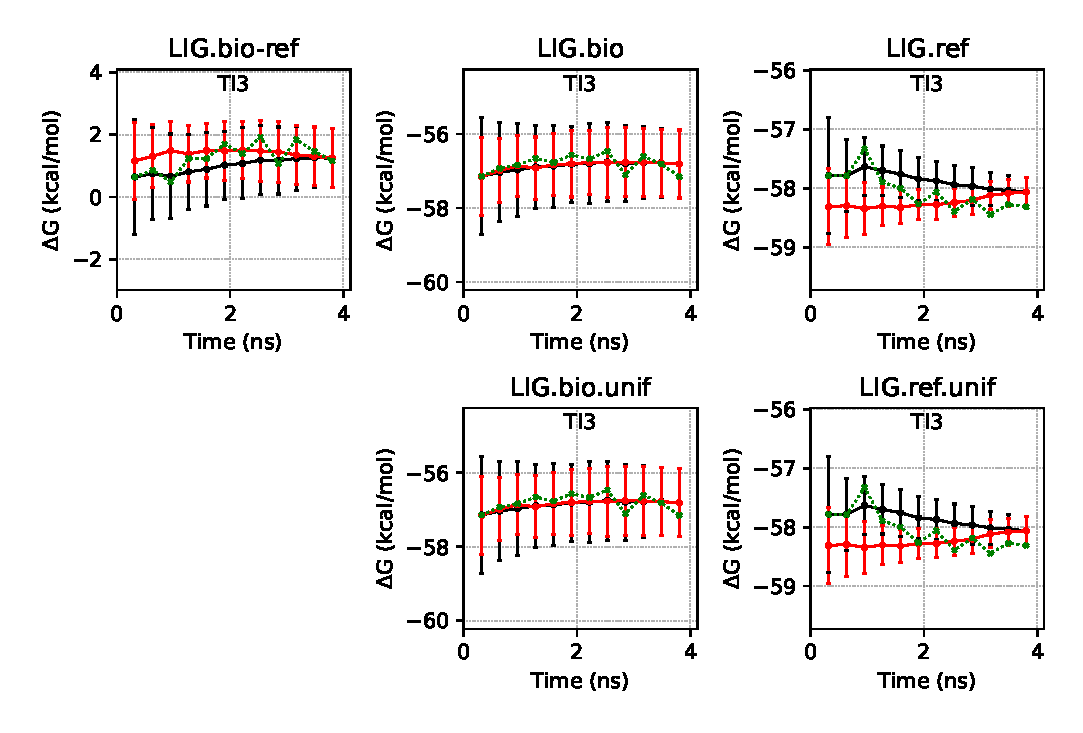
\includegraphics[clip,width=6in]{LIG.bio-ref.GvsT.eps}
\caption{LIG.bio-ref}
\end{figure*}


\clearpage
\pagebreak
\begin{figure*}
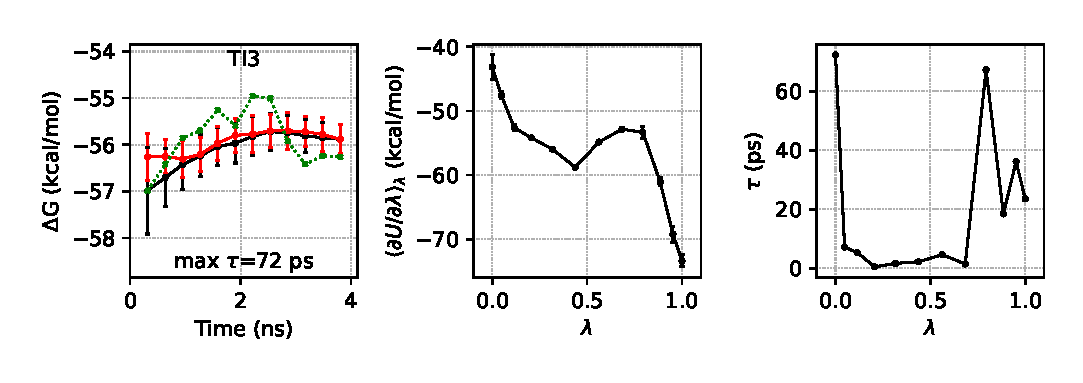
\includegraphics[clip,width=6in]{complex.concerted.t01.results..GvsT.eps}\vspace{-0.3cm}
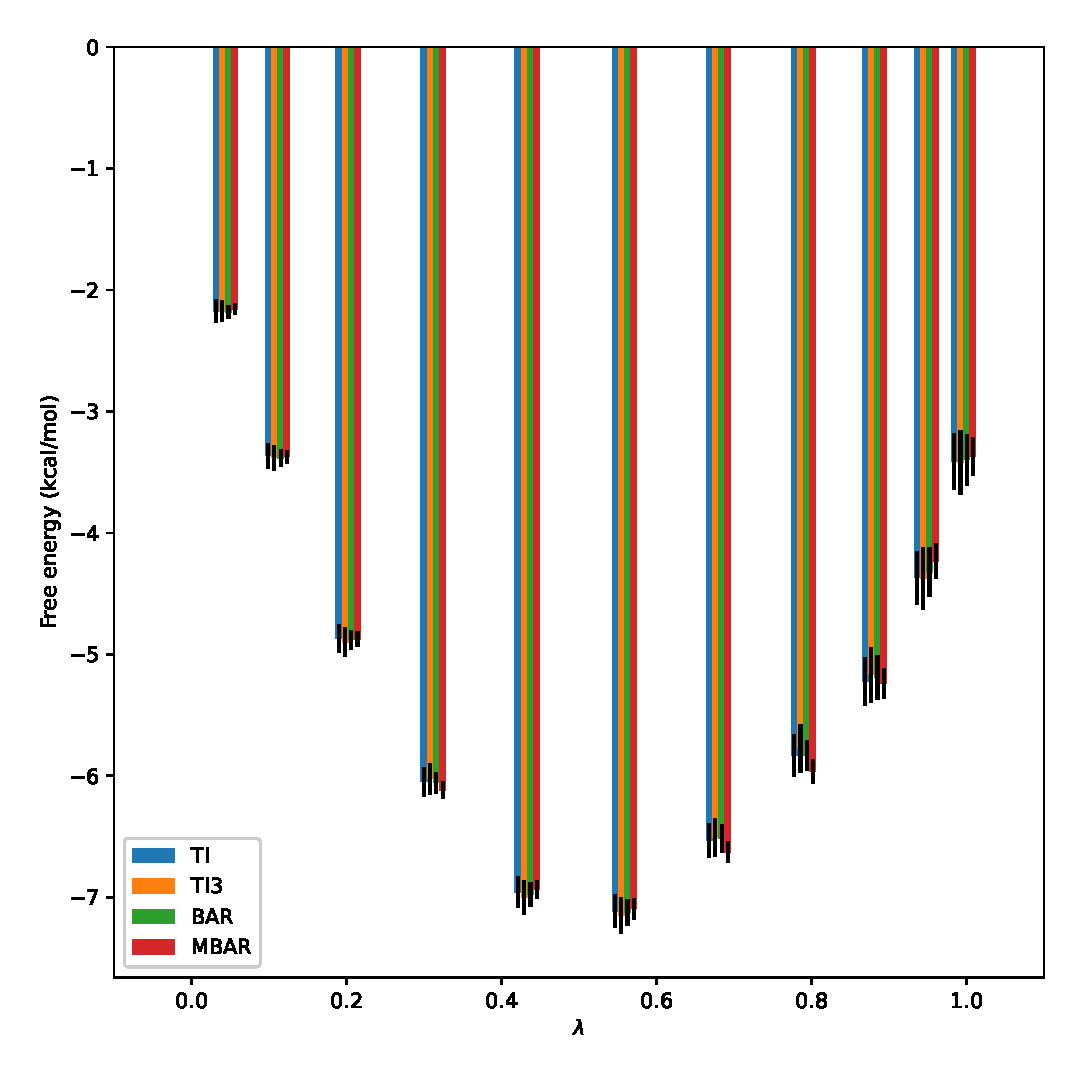
\includegraphics[clip,width=6in]{complex.concerted.t01.results..GvsL.eps}\vspace{-0.3cm}
\caption{LIG.bio.unif.t01 in complex/concerted/t01/results/}
\end{figure*}


\begin{figure*}
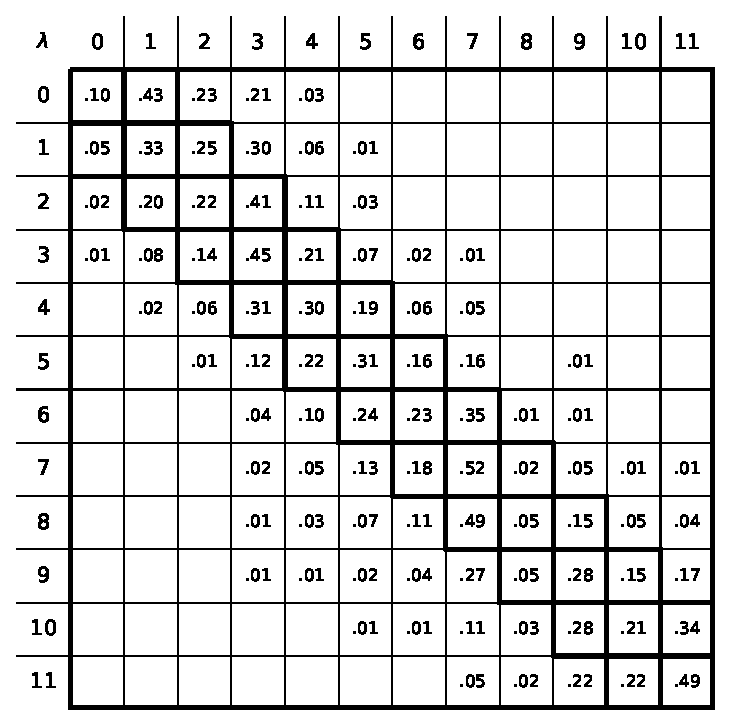
\includegraphics[clip,width=6in]{complex.concerted.t01.results..S.eps}\vspace{-0.3cm}
\caption{MBAR overlap matrix for LIG.bio.unif.t01 in complex/concerted/t01/results/}
\end{figure*}


\begin{figure*}
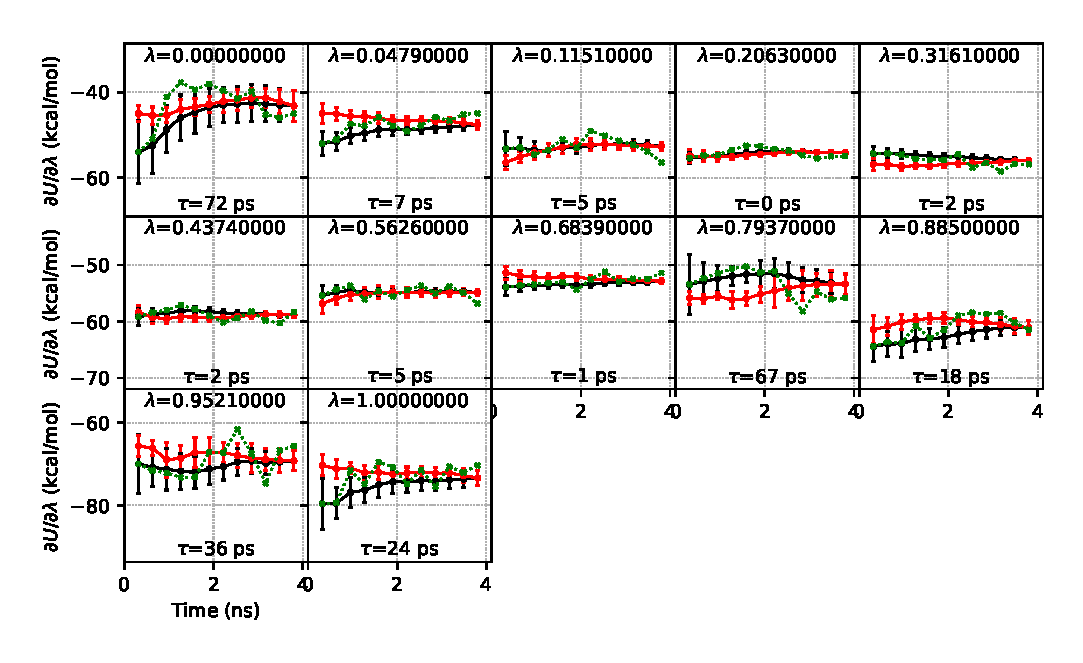
\includegraphics[clip,width=6in]{complex.concerted.t01.results..DVDLvsT.eps}\vspace{-0.3cm}
\caption{$\partial U/\partial\lambda$ time series for LIG.bio.unif.t01 in complex/concerted/t01/results/}
\end{figure*}


\begin{figure*}
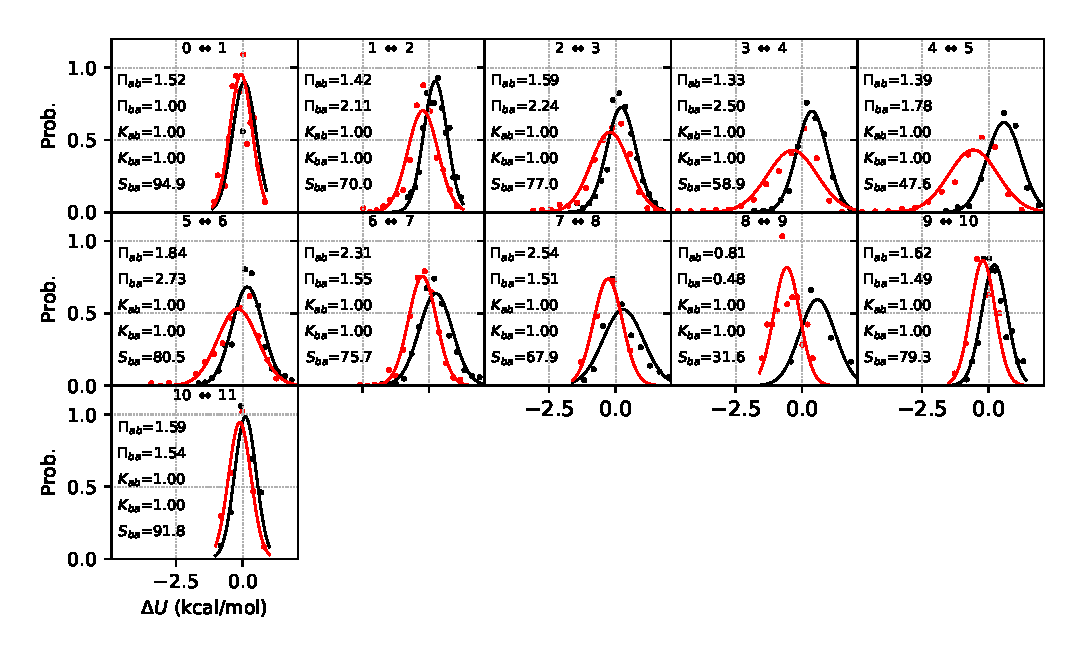
\includegraphics[clip,width=6in]{complex.concerted.t01.results..hist.eps}\vspace{-0.3cm}
                        \caption{Wu and Kofke metrics for LIG.bio.unif.t01 in complex/concerted/t01/results/. The black line is the energy distribution of Ub-Ua from ensemble of a, and the red line is Ua-Ub from the ensemble distribution of b. If the $\Pi$ metrics are negative, then more sampling is likely needed.}
\end{figure*}


\clearpage
\pagebreak
\begin{figure*}
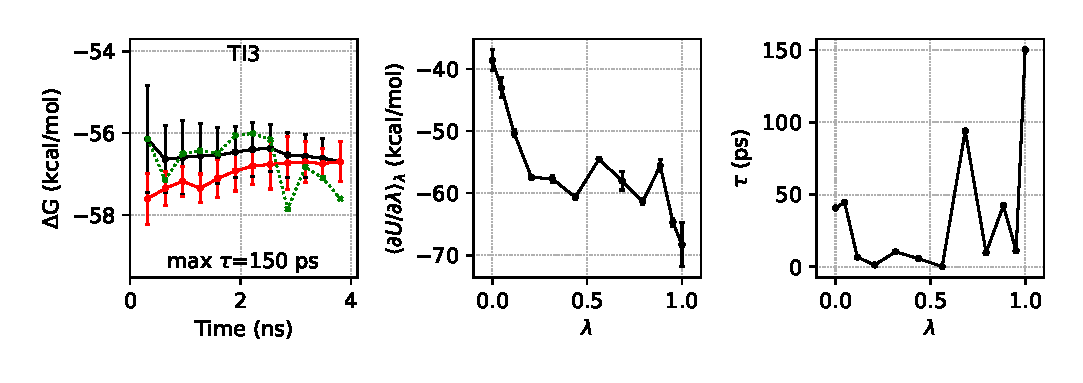
\includegraphics[clip,width=6in]{complex.concerted.t02.results..GvsT.eps}\vspace{-0.3cm}
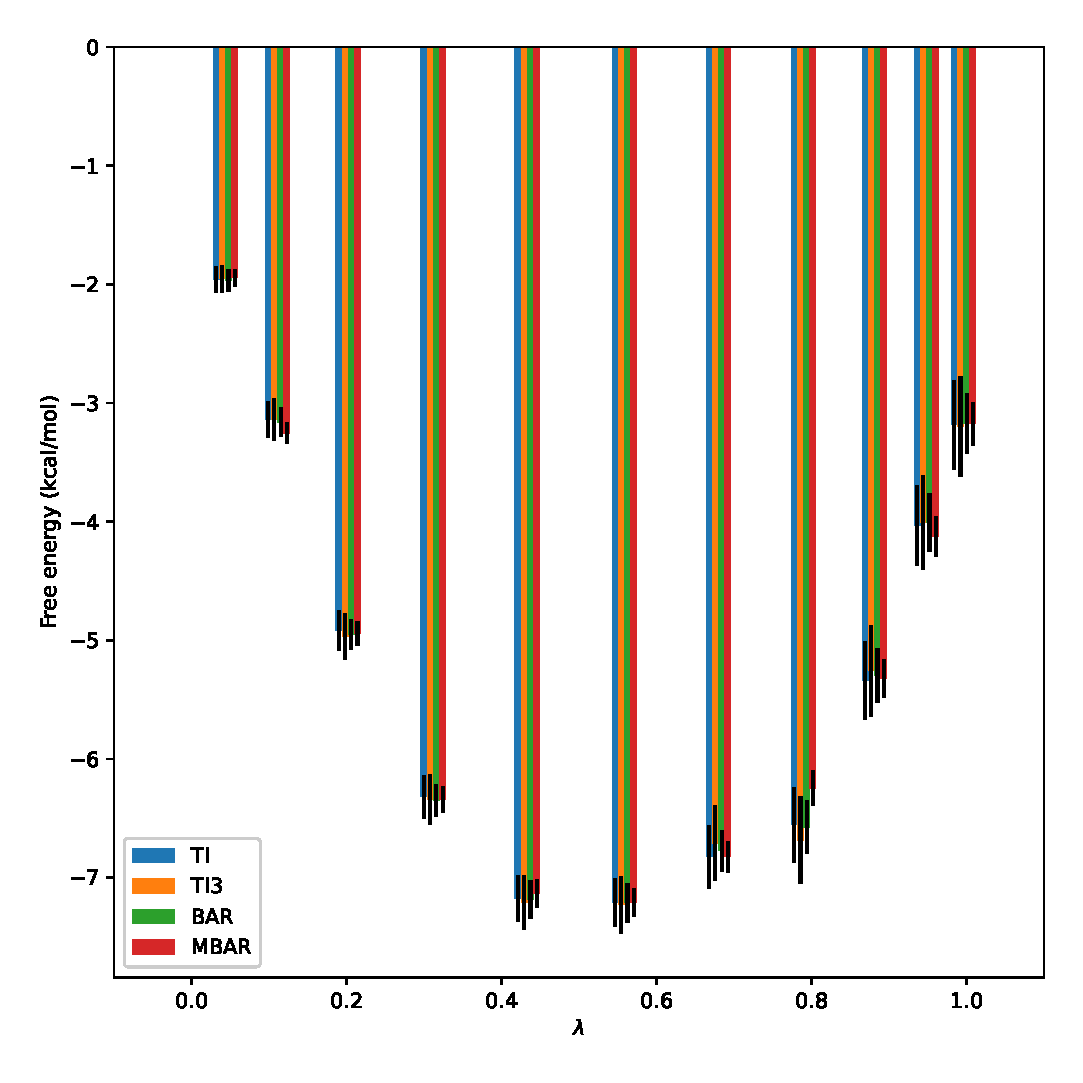
\includegraphics[clip,width=6in]{complex.concerted.t02.results..GvsL.eps}\vspace{-0.3cm}
\caption{LIG.bio.unif.t02 in complex/concerted/t02/results/}
\end{figure*}


\begin{figure*}
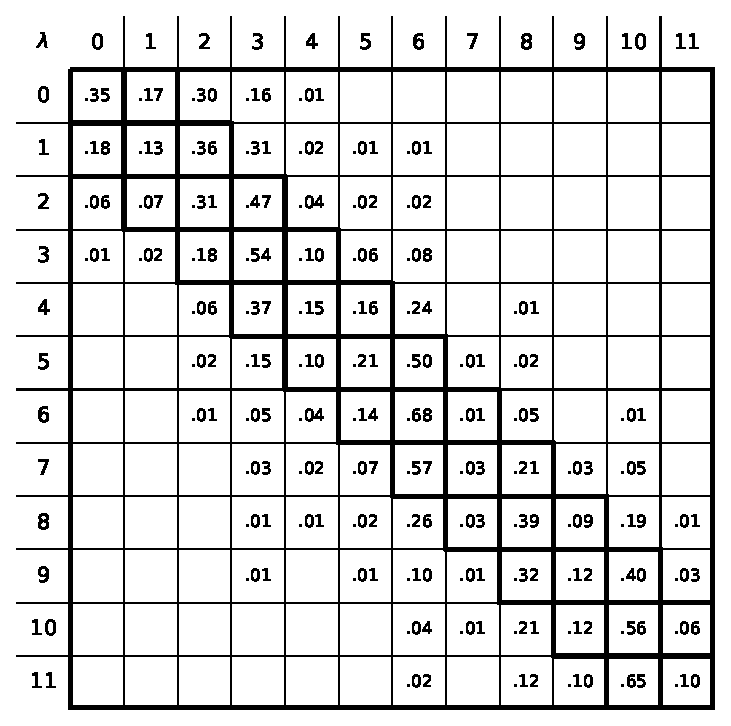
\includegraphics[clip,width=6in]{complex.concerted.t02.results..S.eps}\vspace{-0.3cm}
\caption{MBAR overlap matrix for LIG.bio.unif.t02 in complex/concerted/t02/results/}
\end{figure*}


\begin{figure*}
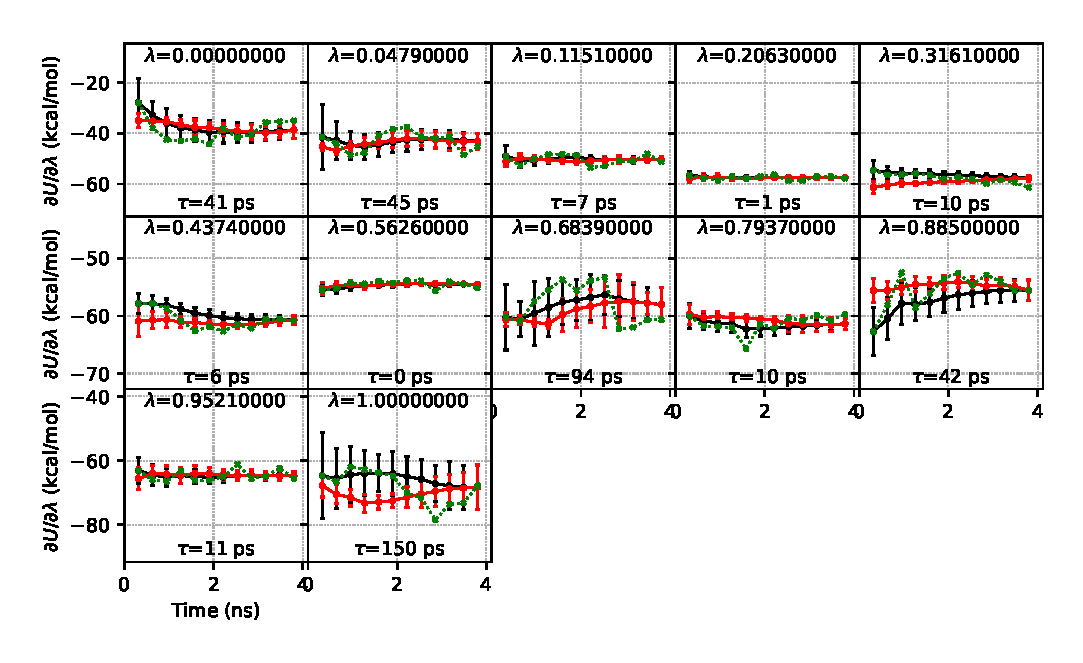
\includegraphics[clip,width=6in]{complex.concerted.t02.results..DVDLvsT.eps}\vspace{-0.3cm}
\caption{$\partial U/\partial\lambda$ time series for LIG.bio.unif.t02 in complex/concerted/t02/results/}
\end{figure*}


\begin{figure*}
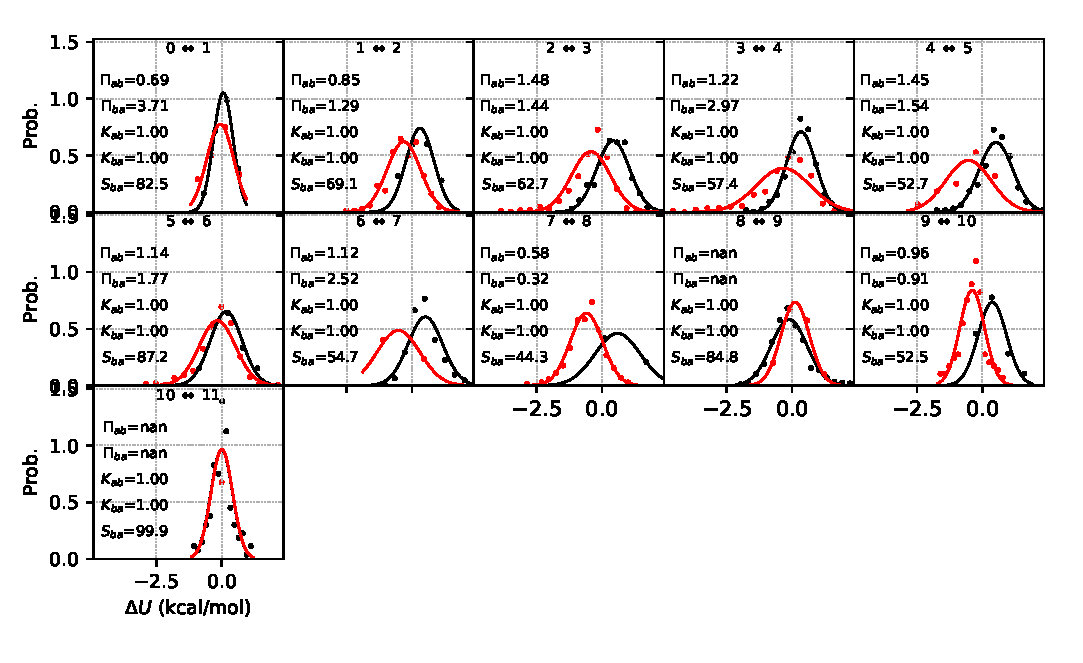
\includegraphics[clip,width=6in]{complex.concerted.t02.results..hist.eps}\vspace{-0.3cm}
                        \caption{Wu and Kofke metrics for LIG.bio.unif.t02 in complex/concerted/t02/results/. The black line is the energy distribution of Ub-Ua from ensemble of a, and the red line is Ua-Ub from the ensemble distribution of b. If the $\Pi$ metrics are negative, then more sampling is likely needed.}
\end{figure*}


\clearpage
\pagebreak
\begin{figure*}
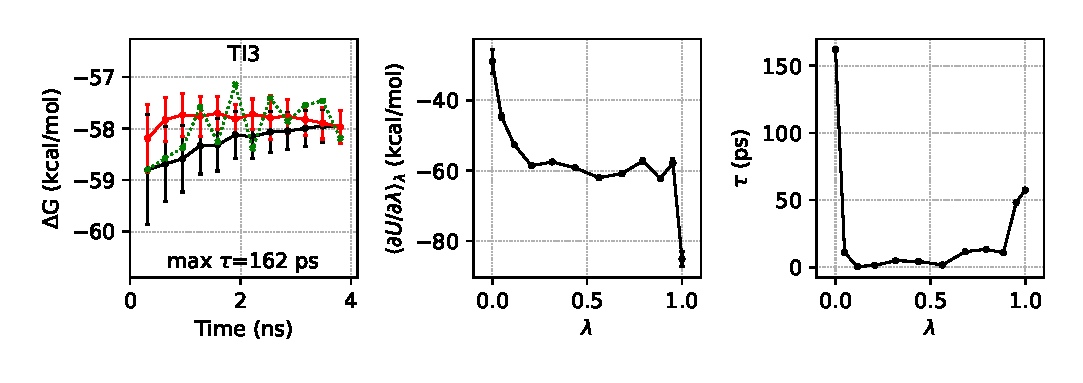
\includegraphics[clip,width=6in]{complex.concerted.t03.results..GvsT.eps}\vspace{-0.3cm}
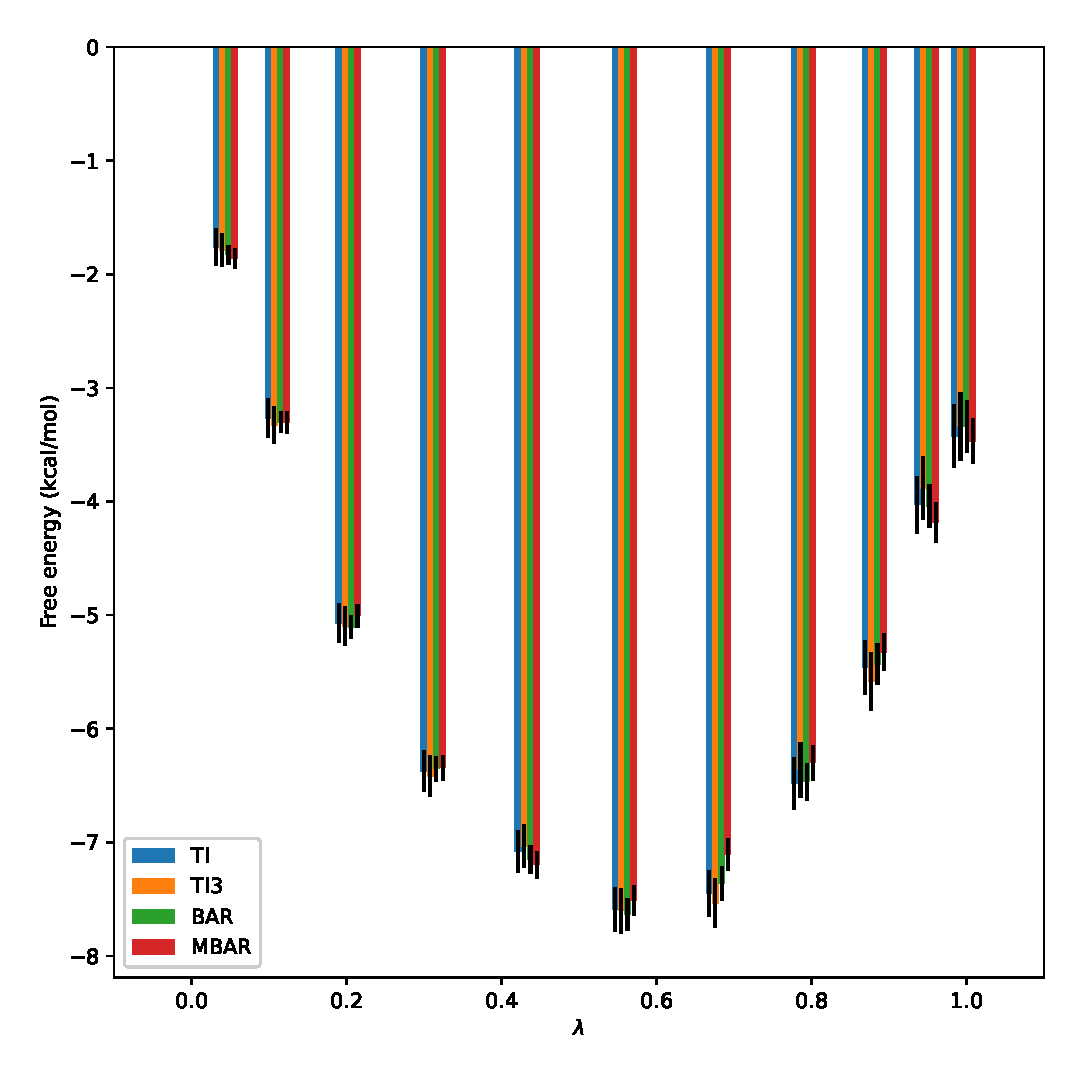
\includegraphics[clip,width=6in]{complex.concerted.t03.results..GvsL.eps}\vspace{-0.3cm}
\caption{LIG.bio.unif.t03 in complex/concerted/t03/results/}
\end{figure*}


\begin{figure*}
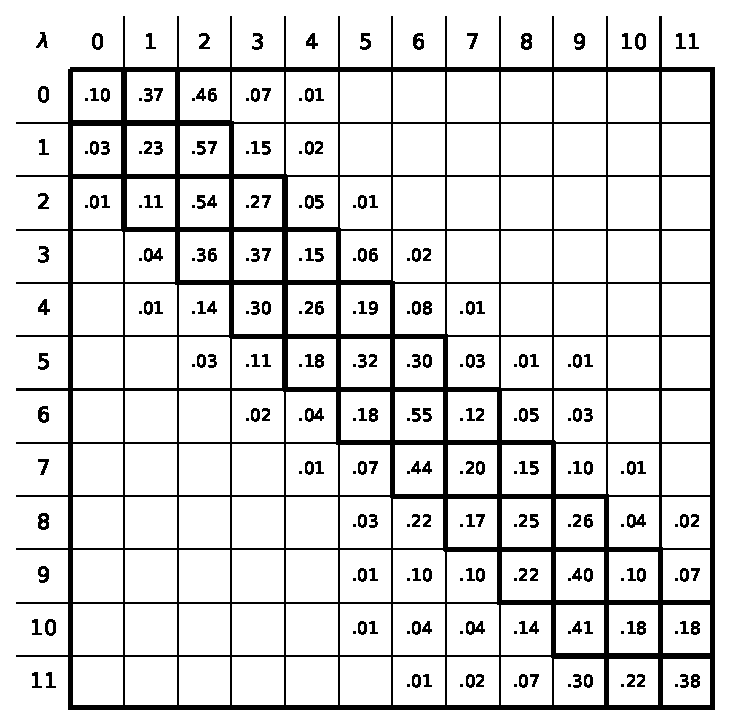
\includegraphics[clip,width=6in]{complex.concerted.t03.results..S.eps}\vspace{-0.3cm}
\caption{MBAR overlap matrix for LIG.bio.unif.t03 in complex/concerted/t03/results/}
\end{figure*}


\begin{figure*}
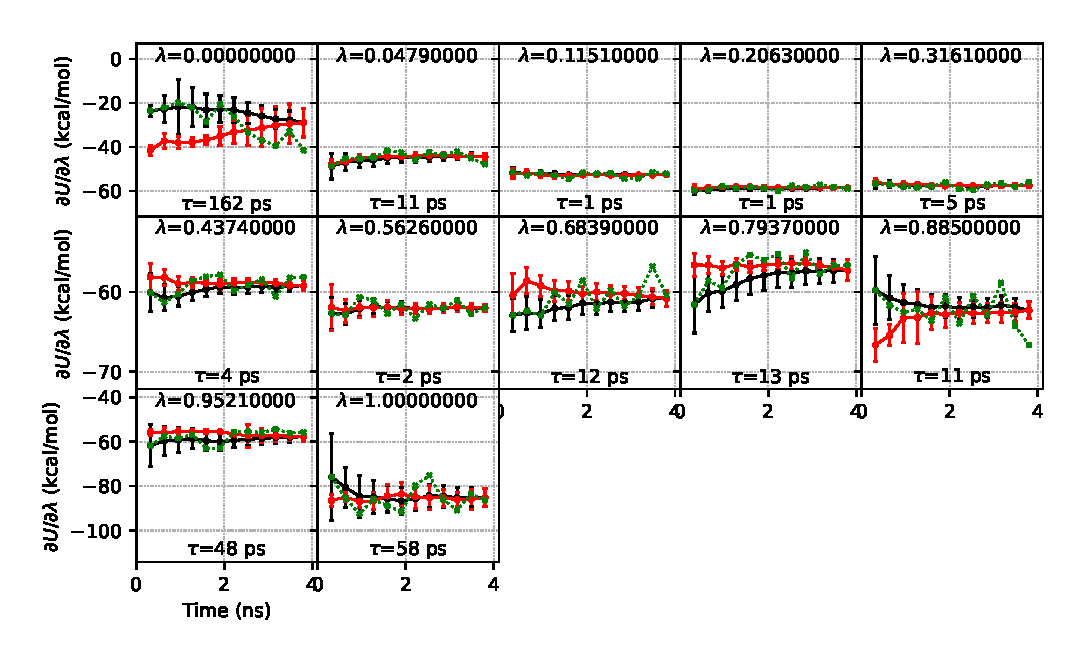
\includegraphics[clip,width=6in]{complex.concerted.t03.results..DVDLvsT.eps}\vspace{-0.3cm}
\caption{$\partial U/\partial\lambda$ time series for LIG.bio.unif.t03 in complex/concerted/t03/results/}
\end{figure*}


\begin{figure*}
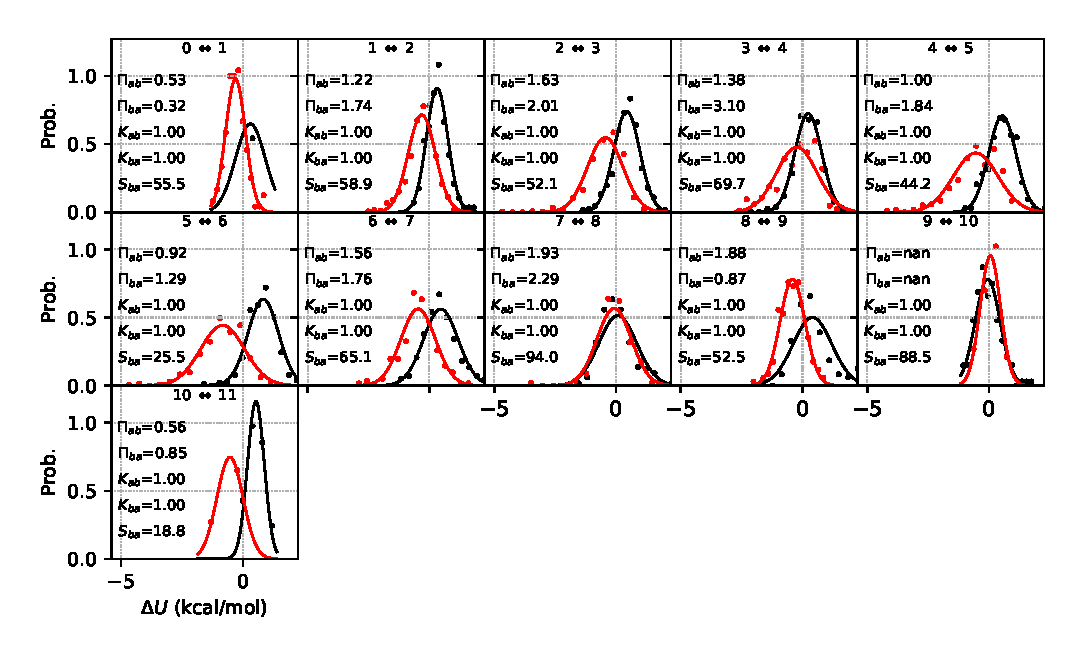
\includegraphics[clip,width=6in]{complex.concerted.t03.results..hist.eps}\vspace{-0.3cm}
                        \caption{Wu and Kofke metrics for LIG.bio.unif.t03 in complex/concerted/t03/results/. The black line is the energy distribution of Ub-Ua from ensemble of a, and the red line is Ua-Ub from the ensemble distribution of b. If the $\Pi$ metrics are negative, then more sampling is likely needed.}
\end{figure*}


\clearpage
\pagebreak
\begin{figure*}
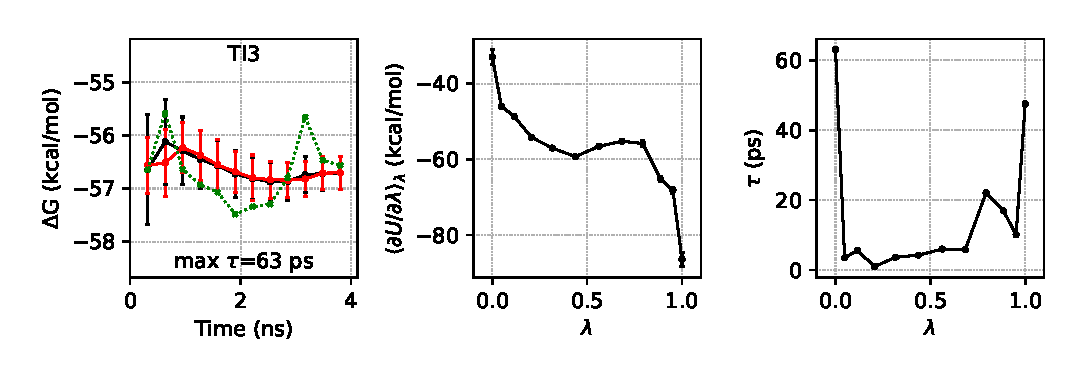
\includegraphics[clip,width=6in]{complex.concerted.t04.results..GvsT.eps}\vspace{-0.3cm}
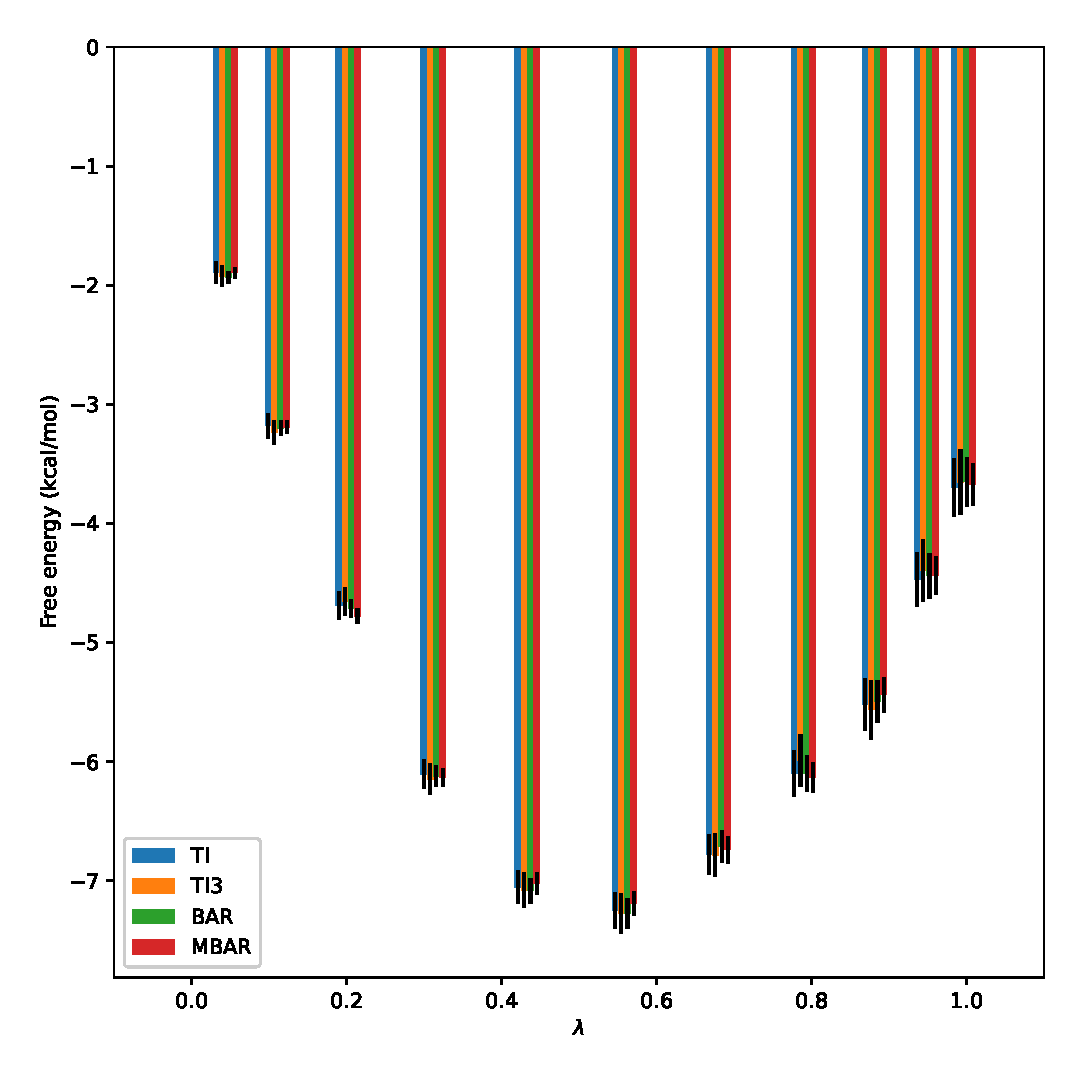
\includegraphics[clip,width=6in]{complex.concerted.t04.results..GvsL.eps}\vspace{-0.3cm}
\caption{LIG.bio.unif.t04 in complex/concerted/t04/results/}
\end{figure*}


\begin{figure*}
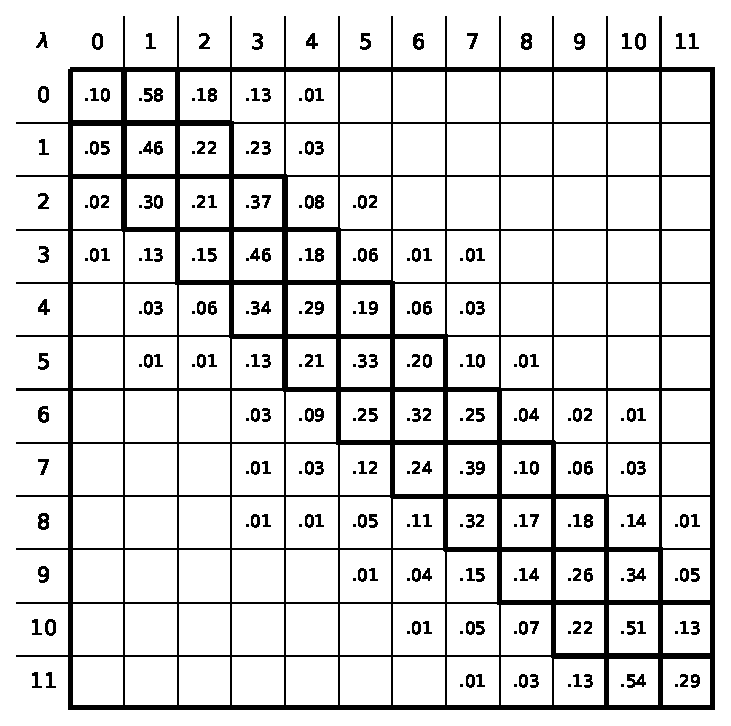
\includegraphics[clip,width=6in]{complex.concerted.t04.results..S.eps}\vspace{-0.3cm}
\caption{MBAR overlap matrix for LIG.bio.unif.t04 in complex/concerted/t04/results/}
\end{figure*}


\begin{figure*}
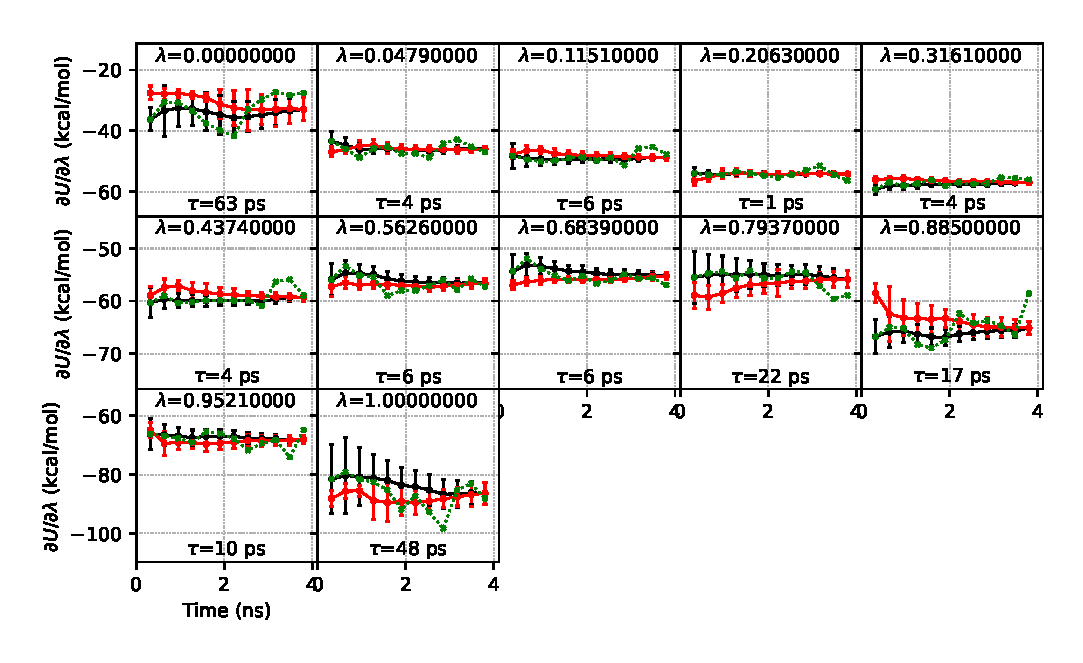
\includegraphics[clip,width=6in]{complex.concerted.t04.results..DVDLvsT.eps}\vspace{-0.3cm}
\caption{$\partial U/\partial\lambda$ time series for LIG.bio.unif.t04 in complex/concerted/t04/results/}
\end{figure*}


\begin{figure*}
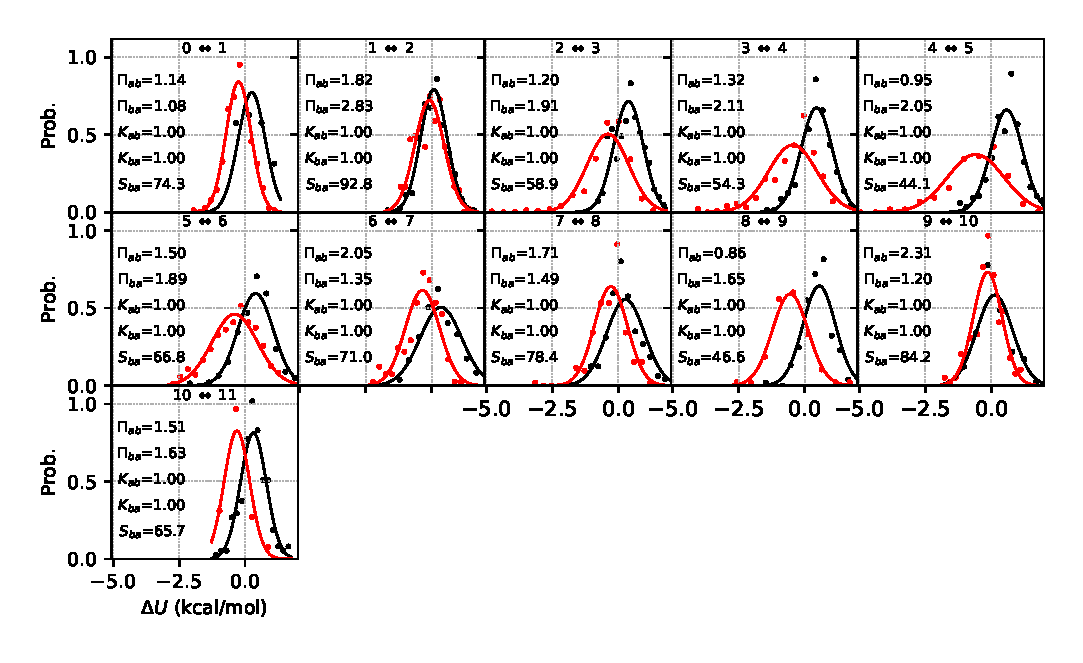
\includegraphics[clip,width=6in]{complex.concerted.t04.results..hist.eps}\vspace{-0.3cm}
                        \caption{Wu and Kofke metrics for LIG.bio.unif.t04 in complex/concerted/t04/results/. The black line is the energy distribution of Ub-Ua from ensemble of a, and the red line is Ua-Ub from the ensemble distribution of b. If the $\Pi$ metrics are negative, then more sampling is likely needed.}
\end{figure*}


\clearpage
\pagebreak
\begin{figure*}
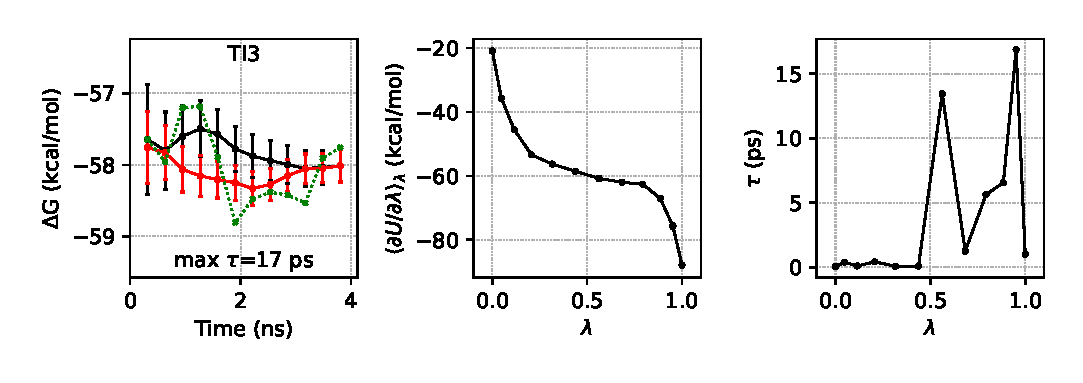
\includegraphics[clip,width=6in]{ligand.concerted.t01.results..GvsT.eps}\vspace{-0.3cm}
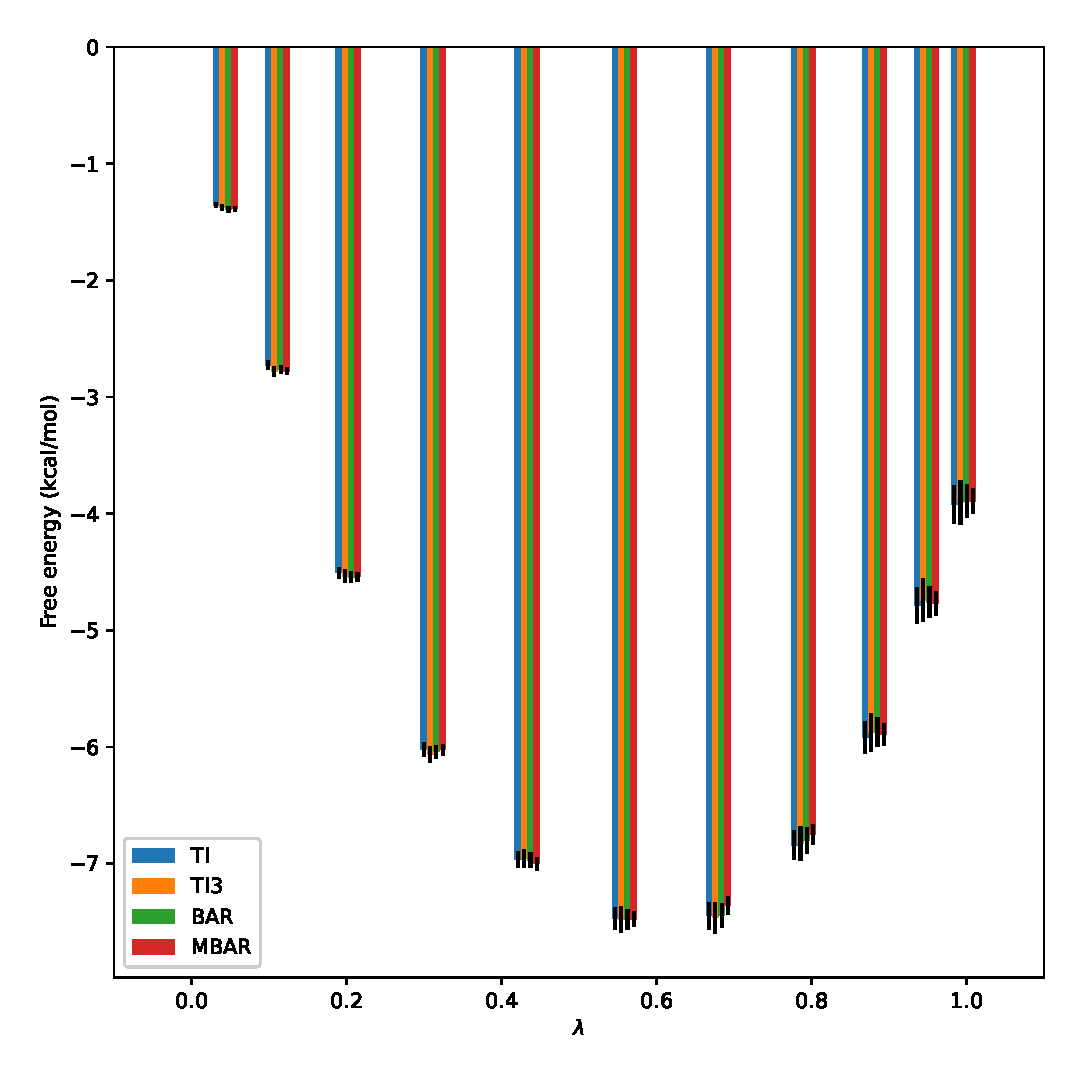
\includegraphics[clip,width=6in]{ligand.concerted.t01.results..GvsL.eps}\vspace{-0.3cm}
\caption{LIG.ref.unif.t01 in ligand/concerted/t01/results/}
\end{figure*}


\begin{figure*}
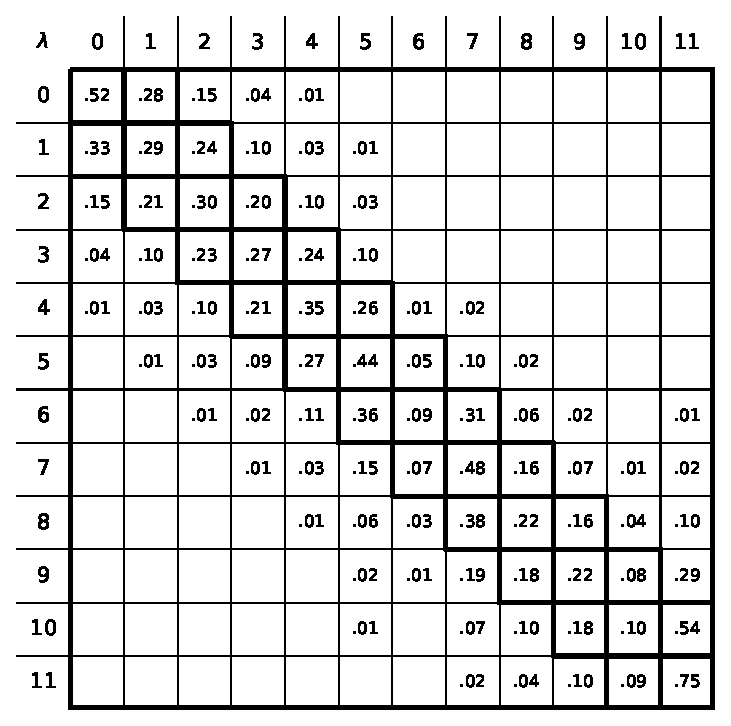
\includegraphics[clip,width=6in]{ligand.concerted.t01.results..S.eps}\vspace{-0.3cm}
\caption{MBAR overlap matrix for LIG.ref.unif.t01 in ligand/concerted/t01/results/}
\end{figure*}


\begin{figure*}
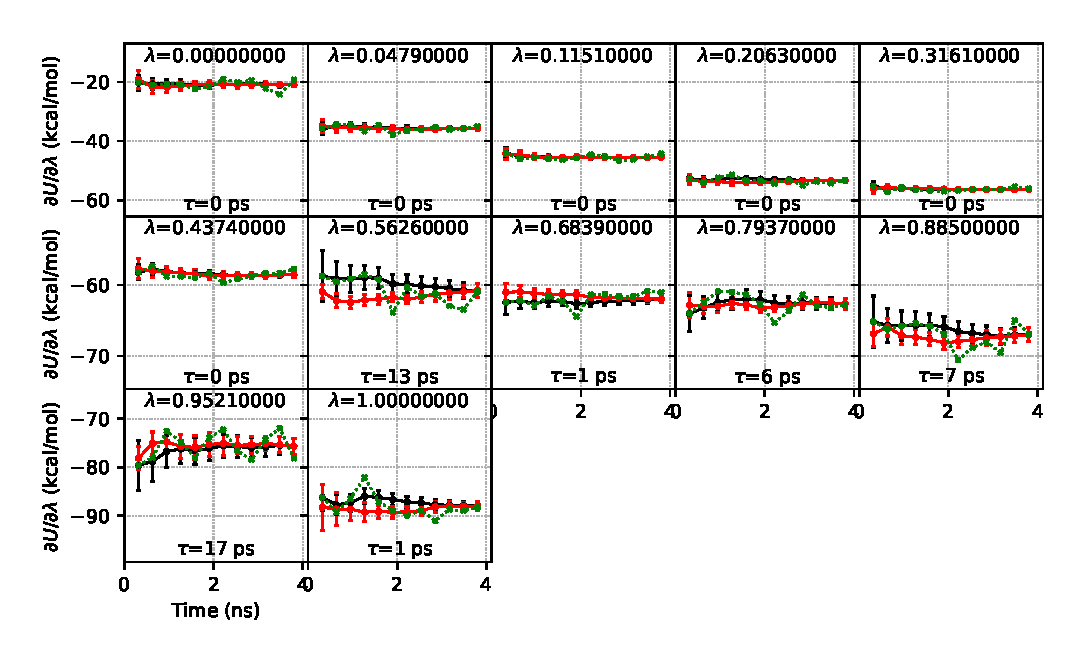
\includegraphics[clip,width=6in]{ligand.concerted.t01.results..DVDLvsT.eps}\vspace{-0.3cm}
\caption{$\partial U/\partial\lambda$ time series for LIG.ref.unif.t01 in ligand/concerted/t01/results/}
\end{figure*}


\begin{figure*}
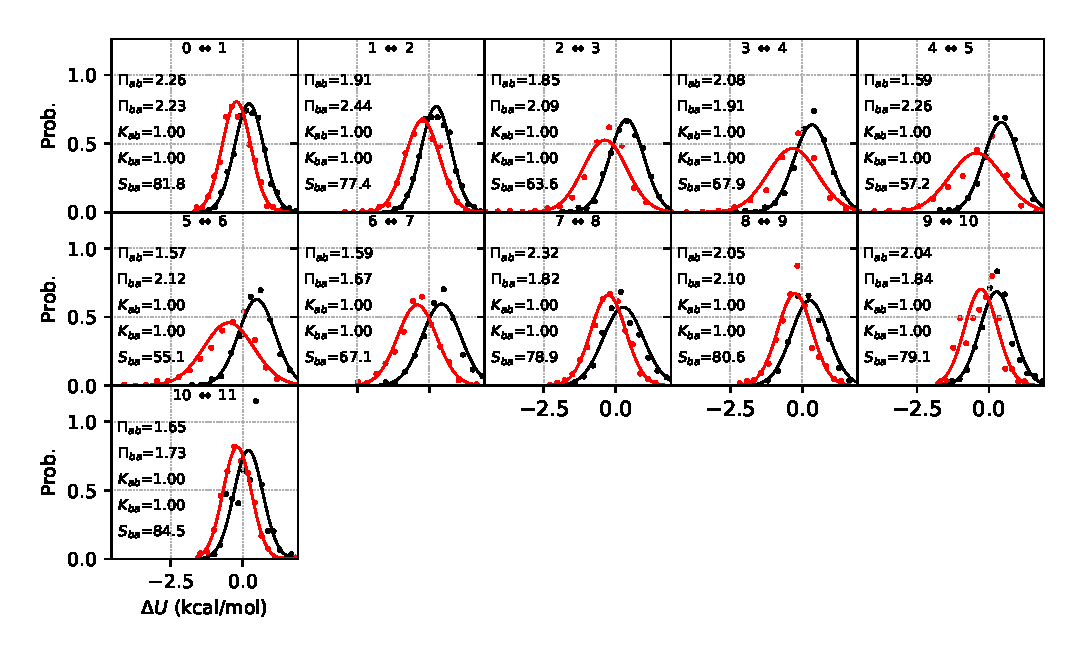
\includegraphics[clip,width=6in]{ligand.concerted.t01.results..hist.eps}\vspace{-0.3cm}
                        \caption{Wu and Kofke metrics for LIG.ref.unif.t01 in ligand/concerted/t01/results/. The black line is the energy distribution of Ub-Ua from ensemble of a, and the red line is Ua-Ub from the ensemble distribution of b. If the $\Pi$ metrics are negative, then more sampling is likely needed.}
\end{figure*}


\clearpage
\pagebreak
\begin{figure*}
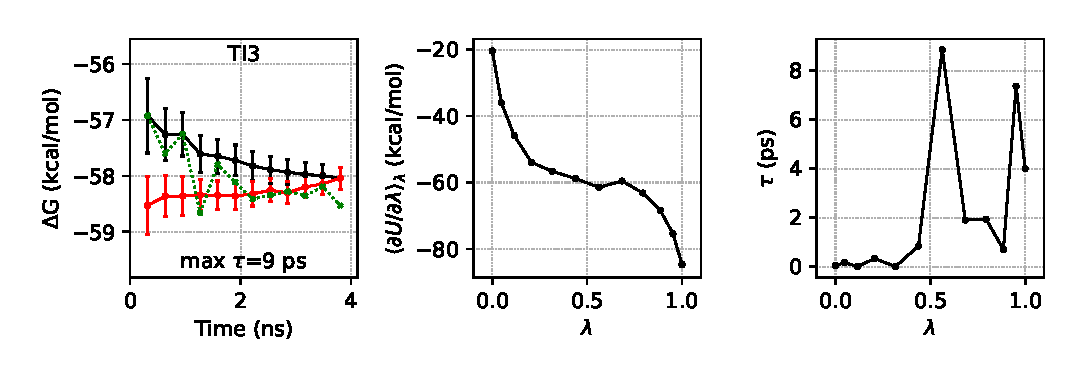
\includegraphics[clip,width=6in]{ligand.concerted.t02.results..GvsT.eps}\vspace{-0.3cm}
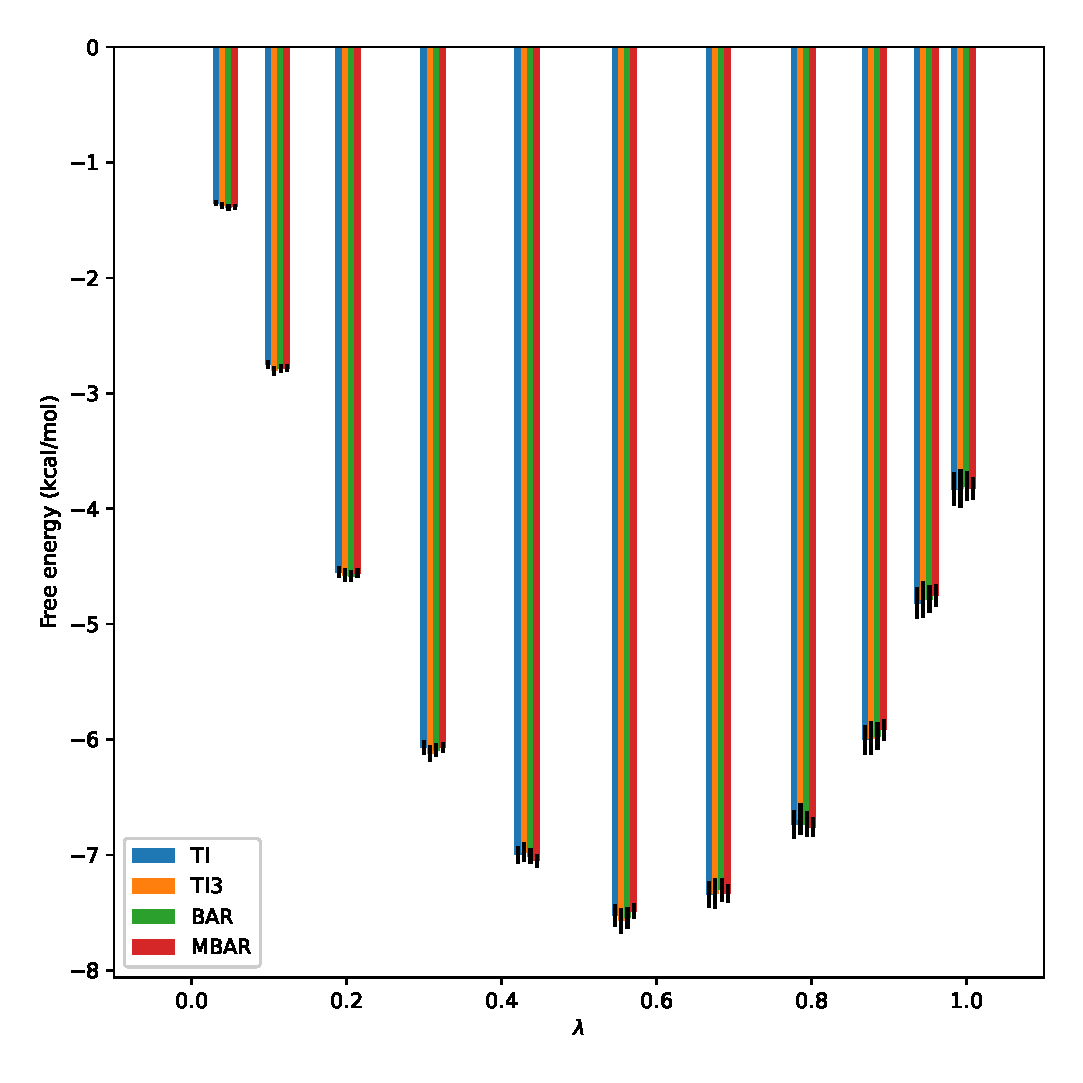
\includegraphics[clip,width=6in]{ligand.concerted.t02.results..GvsL.eps}\vspace{-0.3cm}
\caption{LIG.ref.unif.t02 in ligand/concerted/t02/results/}
\end{figure*}


\begin{figure*}
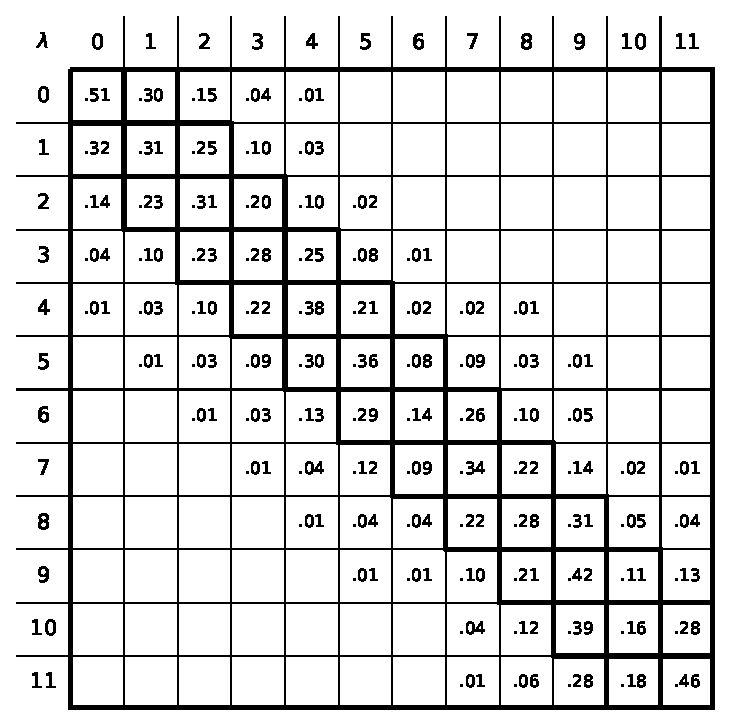
\includegraphics[clip,width=6in]{ligand.concerted.t02.results..S.eps}\vspace{-0.3cm}
\caption{MBAR overlap matrix for LIG.ref.unif.t02 in ligand/concerted/t02/results/}
\end{figure*}


\begin{figure*}
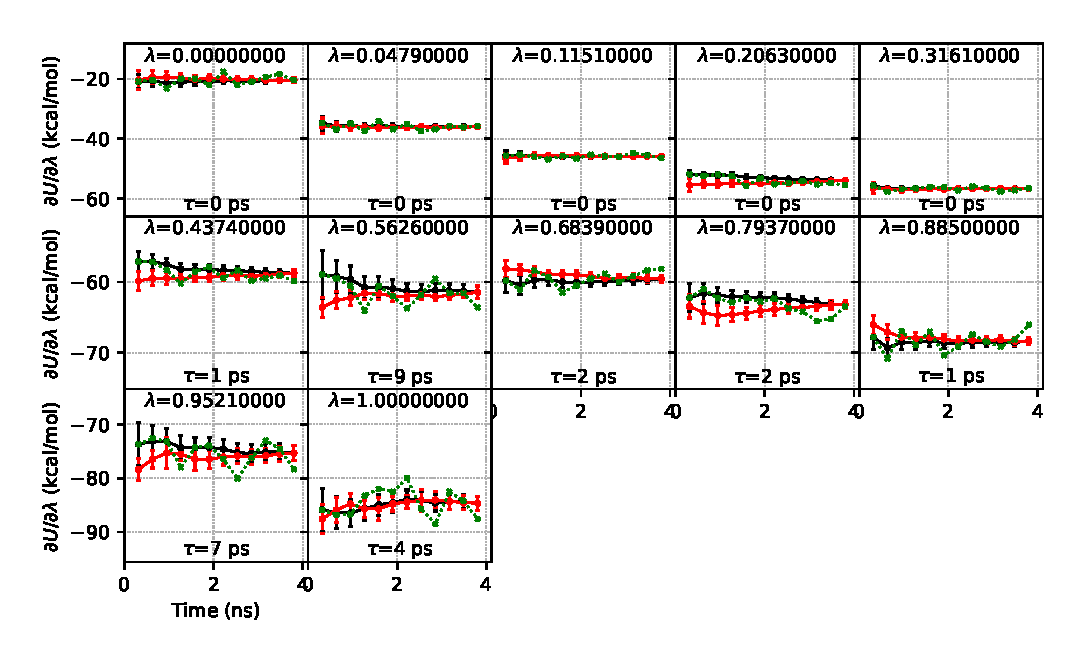
\includegraphics[clip,width=6in]{ligand.concerted.t02.results..DVDLvsT.eps}\vspace{-0.3cm}
\caption{$\partial U/\partial\lambda$ time series for LIG.ref.unif.t02 in ligand/concerted/t02/results/}
\end{figure*}


\begin{figure*}
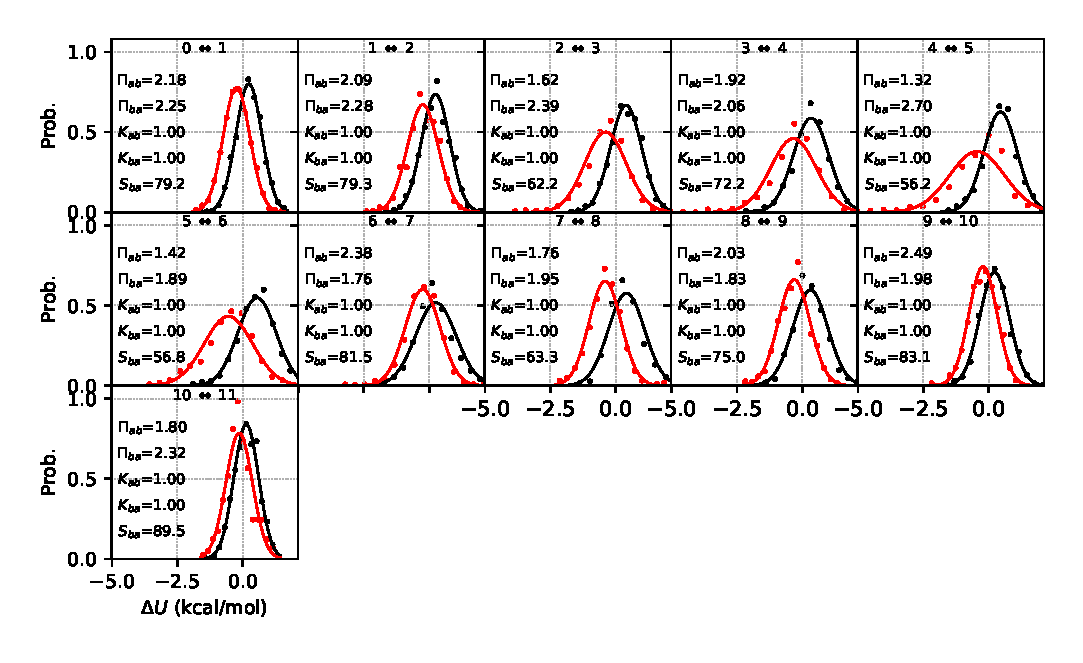
\includegraphics[clip,width=6in]{ligand.concerted.t02.results..hist.eps}\vspace{-0.3cm}
                        \caption{Wu and Kofke metrics for LIG.ref.unif.t02 in ligand/concerted/t02/results/. The black line is the energy distribution of Ub-Ua from ensemble of a, and the red line is Ua-Ub from the ensemble distribution of b. If the $\Pi$ metrics are negative, then more sampling is likely needed.}
\end{figure*}


\clearpage
\pagebreak
\begin{figure*}
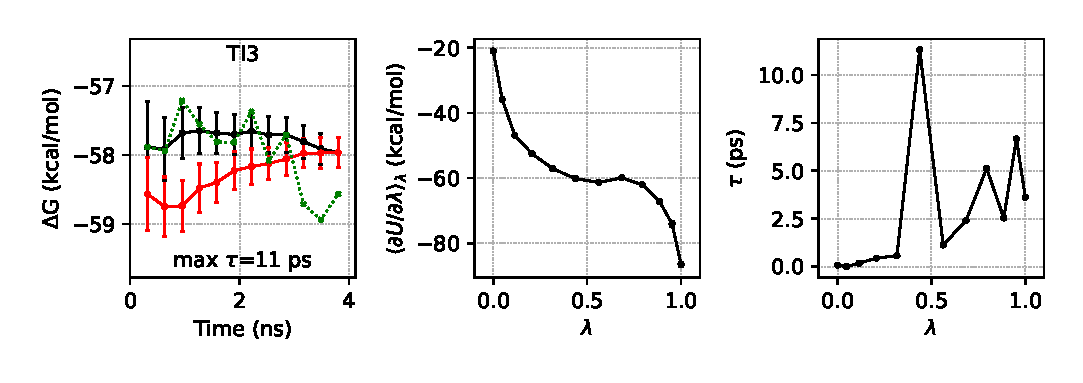
\includegraphics[clip,width=6in]{ligand.concerted.t03.results..GvsT.eps}\vspace{-0.3cm}
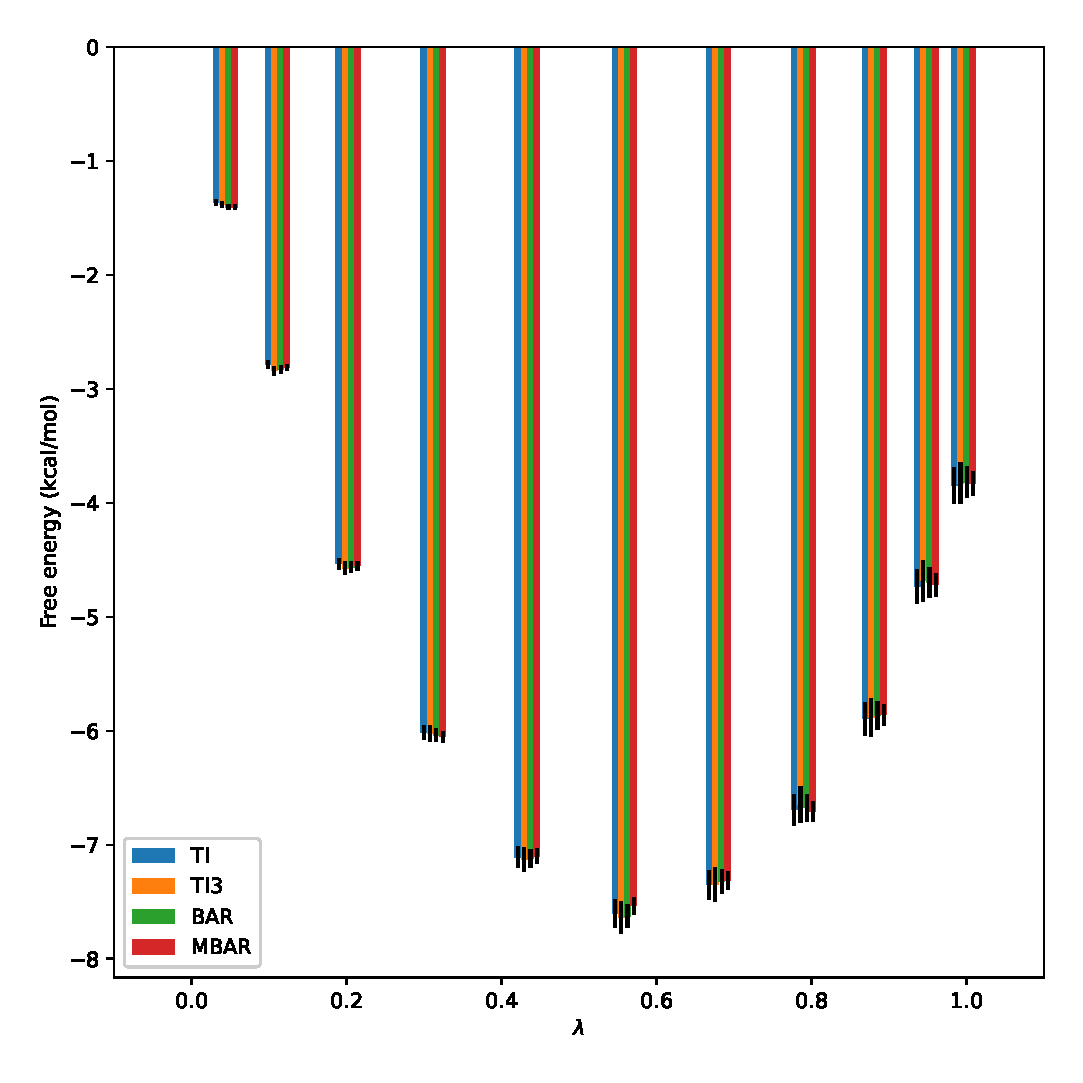
\includegraphics[clip,width=6in]{ligand.concerted.t03.results..GvsL.eps}\vspace{-0.3cm}
\caption{LIG.ref.unif.t03 in ligand/concerted/t03/results/}
\end{figure*}


\begin{figure*}
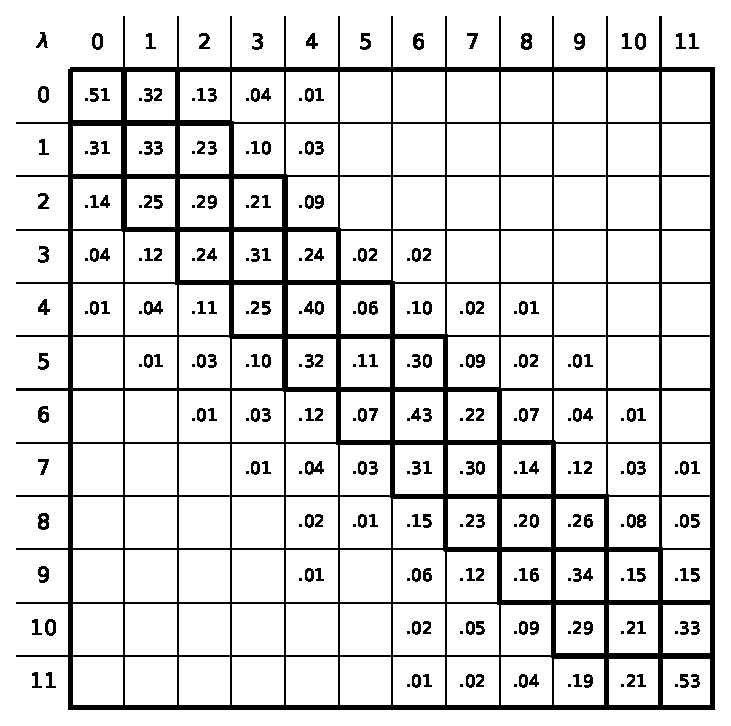
\includegraphics[clip,width=6in]{ligand.concerted.t03.results..S.eps}\vspace{-0.3cm}
\caption{MBAR overlap matrix for LIG.ref.unif.t03 in ligand/concerted/t03/results/}
\end{figure*}


\begin{figure*}
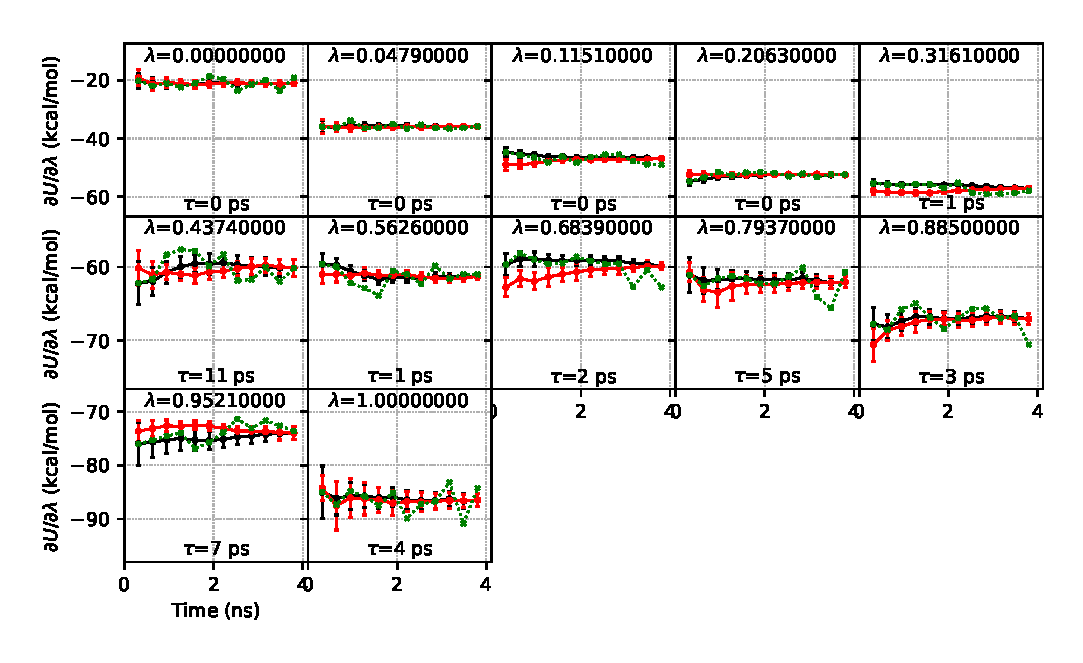
\includegraphics[clip,width=6in]{ligand.concerted.t03.results..DVDLvsT.eps}\vspace{-0.3cm}
\caption{$\partial U/\partial\lambda$ time series for LIG.ref.unif.t03 in ligand/concerted/t03/results/}
\end{figure*}


\begin{figure*}
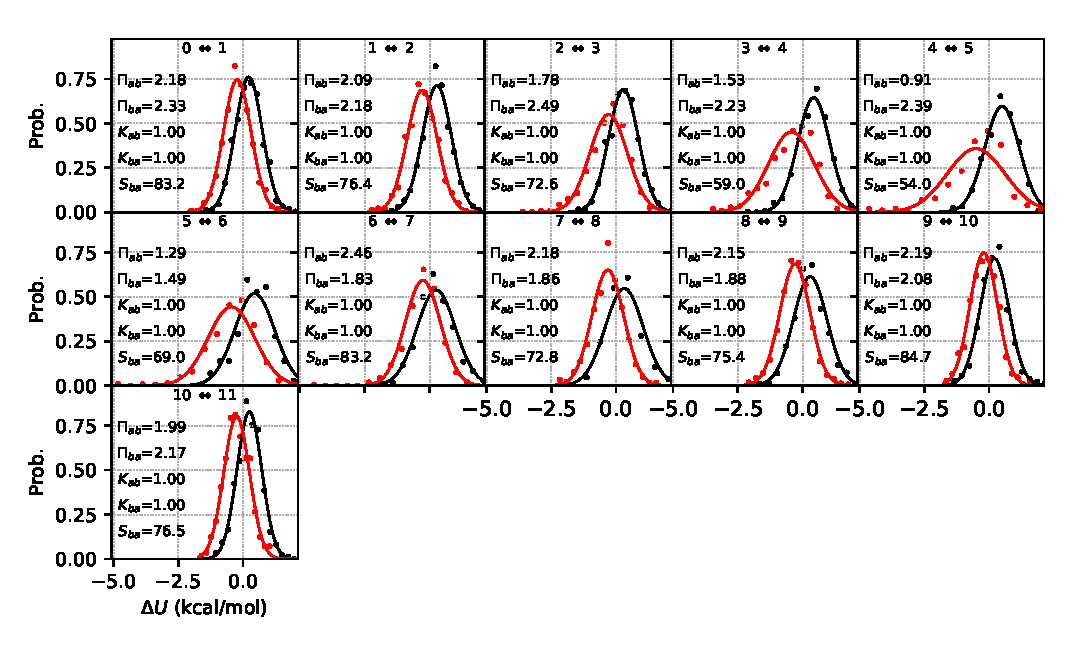
\includegraphics[clip,width=6in]{ligand.concerted.t03.results..hist.eps}\vspace{-0.3cm}
                        \caption{Wu and Kofke metrics for LIG.ref.unif.t03 in ligand/concerted/t03/results/. The black line is the energy distribution of Ub-Ua from ensemble of a, and the red line is Ua-Ub from the ensemble distribution of b. If the $\Pi$ metrics are negative, then more sampling is likely needed.}
\end{figure*}


\clearpage
\pagebreak
\begin{figure*}
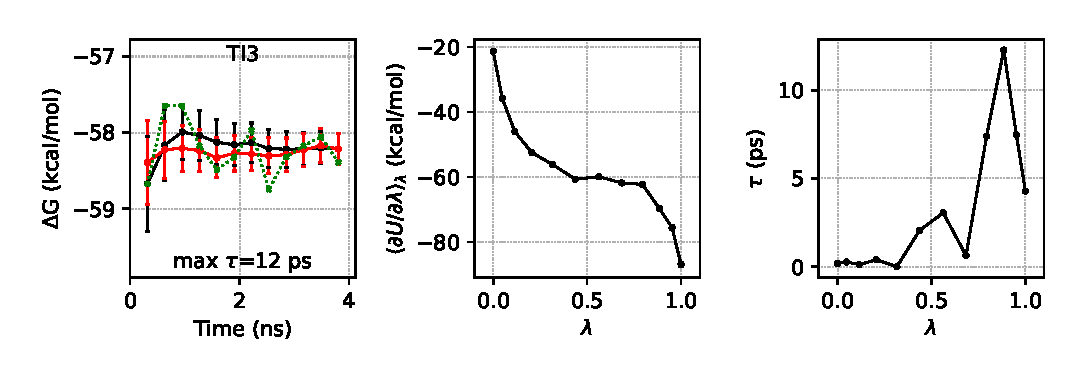
\includegraphics[clip,width=6in]{ligand.concerted.t04.results..GvsT.eps}\vspace{-0.3cm}
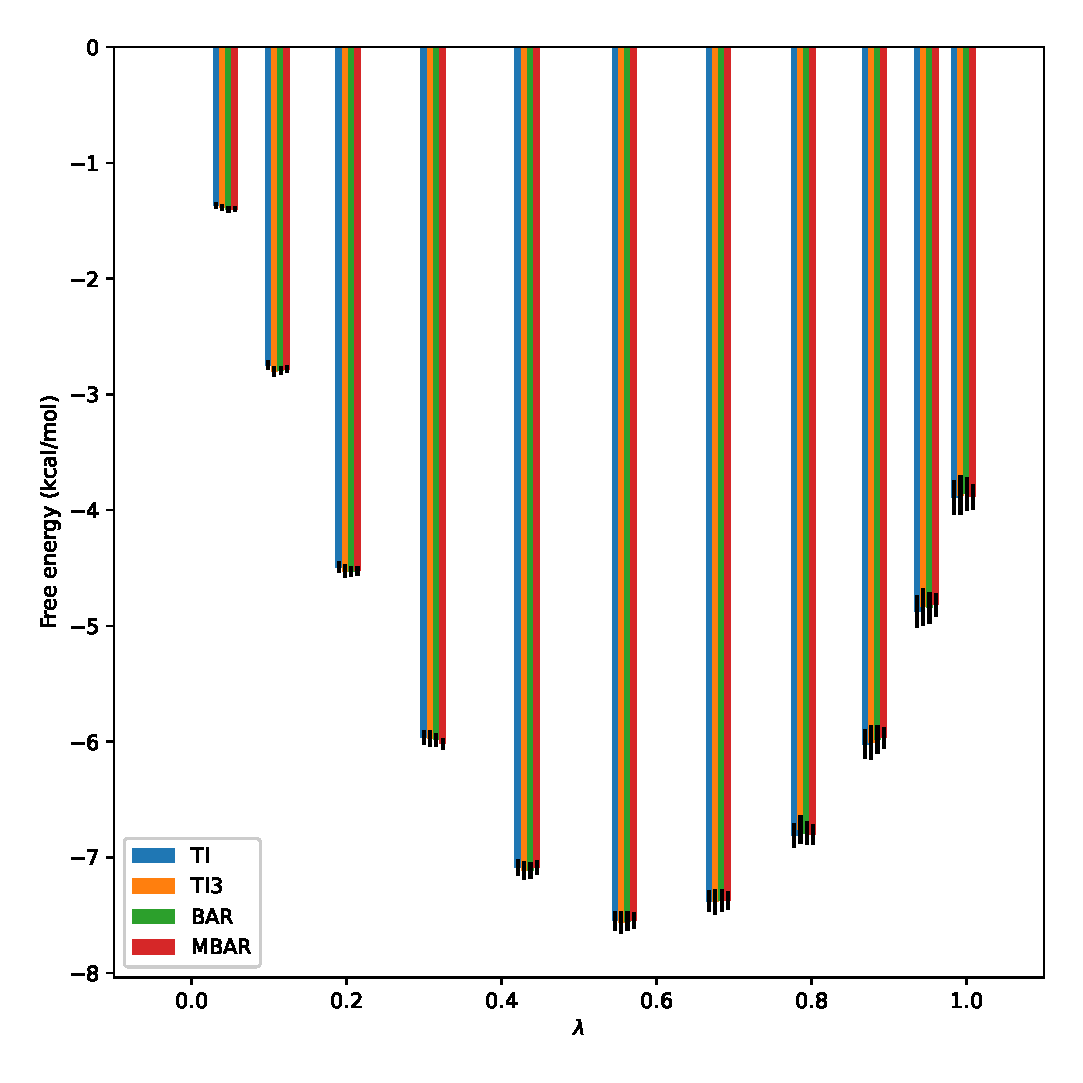
\includegraphics[clip,width=6in]{ligand.concerted.t04.results..GvsL.eps}\vspace{-0.3cm}
\caption{LIG.ref.unif.t04 in ligand/concerted/t04/results/}
\end{figure*}


\begin{figure*}
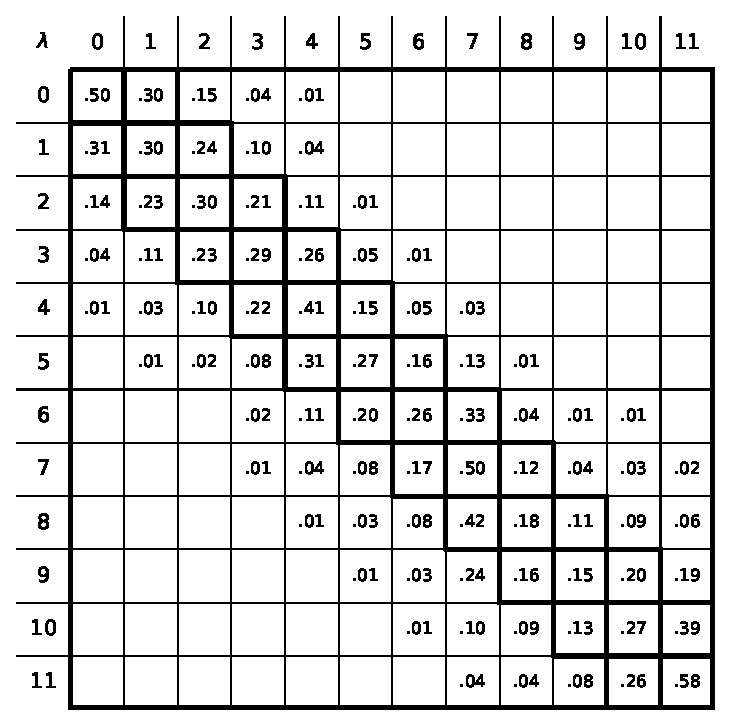
\includegraphics[clip,width=6in]{ligand.concerted.t04.results..S.eps}\vspace{-0.3cm}
\caption{MBAR overlap matrix for LIG.ref.unif.t04 in ligand/concerted/t04/results/}
\end{figure*}


\begin{figure*}
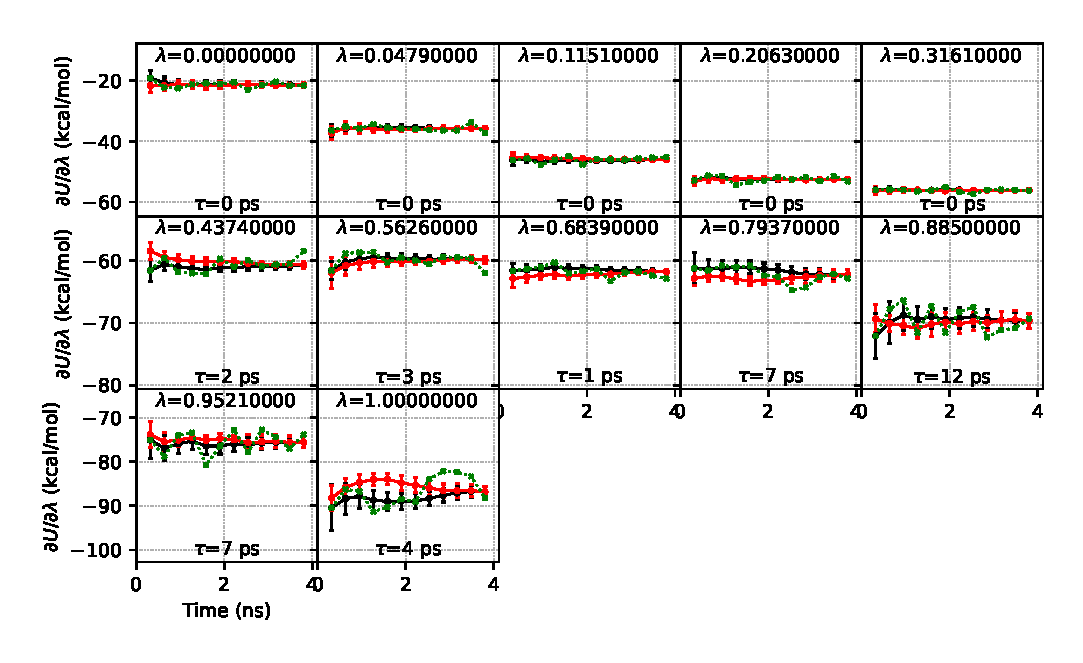
\includegraphics[clip,width=6in]{ligand.concerted.t04.results..DVDLvsT.eps}\vspace{-0.3cm}
\caption{$\partial U/\partial\lambda$ time series for LIG.ref.unif.t04 in ligand/concerted/t04/results/}
\end{figure*}


\begin{figure*}
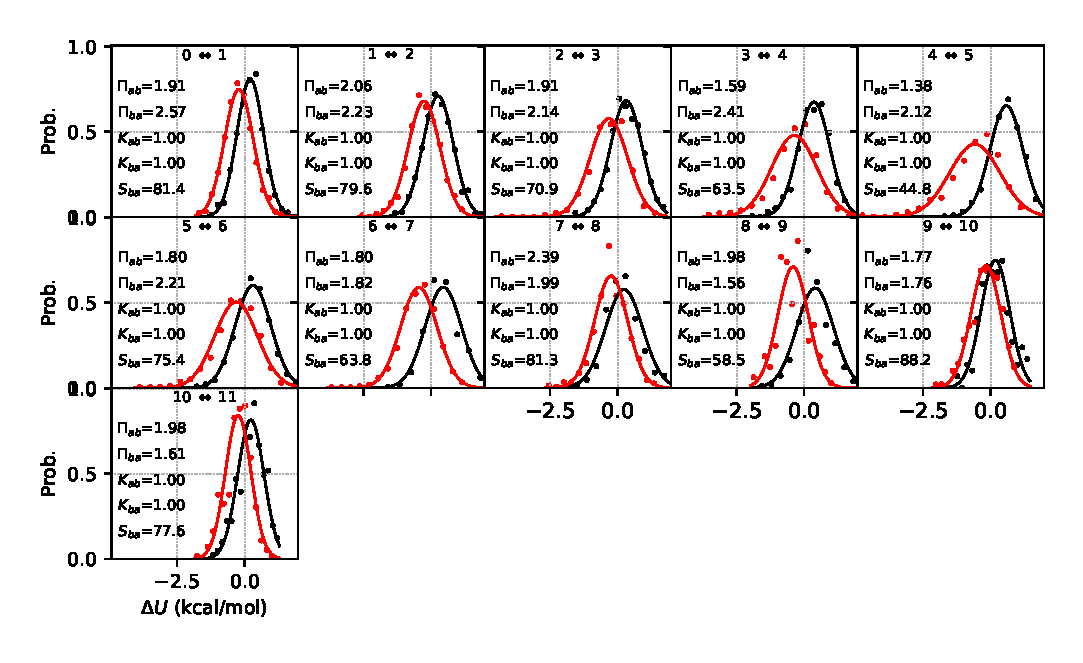
\includegraphics[clip,width=6in]{ligand.concerted.t04.results..hist.eps}\vspace{-0.3cm}
                        \caption{Wu and Kofke metrics for LIG.ref.unif.t04 in ligand/concerted/t04/results/. The black line is the energy distribution of Ub-Ua from ensemble of a, and the red line is Ua-Ub from the ensemble distribution of b. If the $\Pi$ metrics are negative, then more sampling is likely needed.}
\end{figure*}


\clearpage
\pagebreak

\begin{table*}
\caption{Summary, excluding the first 0/12 of the simulations}
{\small
\begin{tabular}{l r r r r r}
\hline
                             Calculation &                 TI &                TI3 &                BAR &               MBAR & max $\tau$\\
\hline                             LIG.bio-ref &    1.19 $\pm$    0.49 &    1.25 $\pm$    0.48 &    1.23 $\pm$    0.47 &    1.28 $\pm$    0.36 &     162 \\

\hline
\end{tabular}
}
\end{table*}

\begin{table*}
\caption{Summary, excluding the first 3/12 of the simulations}
{\small
\begin{tabular}{l r r r r r}
\hline
                             Calculation &                 TI &                TI3 &                BAR &               MBAR & max $\tau$\\
\hline                             LIG.bio-ref &    1.38 $\pm$    0.50 &    1.44 $\pm$    0.50 &    1.43 $\pm$    0.46 &    1.46 $\pm$    0.37 &     110 \\

\hline
\end{tabular}
}
\end{table*}

\begin{table*}
\caption{Summary, excluding the first 4/12 of the simulations}
{\small
\begin{tabular}{l r r r r r}
\hline
                             Calculation &                 TI &                TI3 &                BAR &               MBAR & max $\tau$\\
\hline                             LIG.bio-ref &    1.40 $\pm$    0.50 &    1.47 $\pm$    0.50 &    1.45 $\pm$    0.47 &    1.48 $\pm$    0.37 &     103 \\

\hline
\end{tabular}
}
\end{table*}

\begin{table*}
\caption{Summary, excluding the first 6/12 of the simulations}
{\small
\begin{tabular}{l r r r r r}
\hline
                             Calculation &                 TI &                TI3 &                BAR &               MBAR & max $\tau$\\
\hline                             LIG.bio-ref &    1.40 $\pm$    0.48 &    1.47 $\pm$    0.48 &    1.45 $\pm$    0.46 &    1.49 $\pm$    0.36 &      80 \\

\hline
\end{tabular}
}
\end{table*}
\end{document}

